\documentclass[12pt]{report}
\usepackage[utf8]{inputenc}
\usepackage{amsmath,fullpage,amsfonts,amssymb,tikz,booktabs,geometry,amsthm,pgfplots,relsize,graphicx}
\usepackage[boxruled]{algorithm2e}
\geometry{margin=1in}
\usetikzlibrary{matrix}
\pgfplotsset{soldot/.style={color=blue,only marks,mark=*}} \pgfplotsset{holdot/.style={color=blue,fill=white,only marks,mark=*}}
\usepackage{hyperref}
\usepackage{setspace}
\doublespacing
\title{Scaling MCMC methods for Bayesian neural networks}
\author{Yiu Sing Lau}
\date{}
\begin{document}

\maketitle

\renewcommand{\abstractname}{ACKNOWLEDGEMENTS}
\begin{abstract}
Thank you very much

\end{abstract}

\renewcommand{\abstractname}{ABSTRACT}

\begin{abstract}
Neural network models have seen tremendous success in predictive tasks in machine learning and artificial intelligence(quote), with some attributing their success to the use bayesian inference \cite{mandt2017stochastic}. STAN is a state of the art software for Bayesian statistical computing used mainly in the statistical community, however, it is not optimzed for use with neural network models. In this thesis, we replicated much of STAN's No U-Turn sampler in PyTorch and explore its use for sampling from Bayesian neural network models. We were able to explore different samplers,model structures and their sampling and predictive performances, on a benchmark classification task. We found that Bayesian inference improves predictive performance in general but care is needed with the choice of prior and MCMC sampler. 

\end{abstract}
\tableofcontents 

\chapter{Introduction}
\section{STAN}

STAN has replaced most Bayesian statistical softwares like JAGS and WINBUGS as the recommended tool for Bayesian inference requiring Markov Chain Monte Carlo (MCMC)  because of its effectiveness, relative ease to learn, clear and extensive documentation, as well as its large community of users and expert support staff. Roughly based on the NUTS sampler, it has since evolved from the original NUTS sampler and has many more features built in to facilitate sampling and diagnosing sampling issues.

In Chapter 2, after giving a short introduction to MCMC, we will give an overview of Hamiltonian Monte Carlo, which is the foundation on which NUTS is built. Then we will explain the version of No U-TURN Sampler (NUTS) implemented in STAN, highlighting its difference from the original implemnted in \cite{hoffman2014no}. The exhasutive terminal criteiron for NUTS (XHMC) , which has not been exposed in the latest version of STAN yet, has been shown to improve sampling efficiency in correlated distributions.  \cite{betancourt2016identifying}. Experiments comparing its performance against the default termination criterion will be discussed in chapter 4. Then we review the automatic tuning strategies for the step size parameter and covariance metric used by STAN, followed by a discussion of the built-in convergence diagnostics, NUTS-specific and otherwise.
Finally, we discuss some of the numerical tricks used by STAN that are omitted in the official documentation but can be critical for creating a robust implementation. 

Most algorithms discussed in chapter 2 will come with clear pseudocode and have been implemented. 






\section{Bayesian Neural Network }

Neural network models have become hugely popular under the name of Deep Learning, attracting a lot of attention from researchers and practitioners alike. Many of its successes come from applications in vision, text, speech, and many other sub-fields in the field of Artificial Intelligence. Although there is no yet a consensus that explains why these models do so well, in many cases defying existing learning theory. 


In Chapter 3 we give a brief overview of the Bayesian neural network literature and identify areas where we feel could benefit from new developments in NUTS and related sampling techniques. In Neal's and Cho's work \cite{neal1993bayesian,choo2000learning}, sampling from the posterior distribution was done by alternating between the lower and higher level parameters in a block-Gibbs fashion. With the model and data they used, they found that joint sampling offered no improvement over Gibbs sampling for sampling the hyperparameter. We found that NUTS is capable of sampling the hyperparameter quite well, is more robust to tuning parameters, and requires much less manual tuning. 

Then we talk about the choice of prior for neural network models. Originally it was standard to put a hierarchical prior on the model weights, but in the new wave of Bayesian deep learning literature the standard normal prior is used most of the times. Recently shrinkage priors like the horseshoe prior have been used to automatically regularize the weights \cite{ghosh2017model}. In their paper the authors used variational inference to approximate the predictive distribution, which might miss important features of the  distribution. We used NUTS to perform full posterior inference on a range of shrinkage priors. Basically we found that the standard normal prior performed best in terms of both effective sample size and predictive accuracy. The results of these experiments in full details will be presented in Chapter 4.

While the use of shrinkage priors should eliminate much of the need for model selection: one would simply fit the largest model possible and let the shrinkage prior eliminate any excess capacity, in practice sampling from such a model might prove too difficult, for example having too many hidden layers might result in vanishing or exploding gradients \cite{bengio1994learning}. There are also tuning parameters, like the activation function, which can not be chose by shrinkage priors. This necessitates model selection techniques. Model selection by information criteria like AIC and BIC is not backed by theory because neural networks violate one of their regularity conditions, namely that the model must have non-singular Fisher matrix. The Watanabe Information Criterion (WAIC) is designed to overcome this problem for all singular models. We experimented with the WAIC but found that it failed to choose the model that minimizes the test error on the dataset we chose. 

We also experimented with Stochastic Gradient Hamiltonian Monte Carlo (SGHMC), a version of Hamiltonian Monte Carlo that only uses a fraction of the data to approximate the gradient of the full posterior density function. In \cite{betancourt2015fundamental} the author showed that stochastic gradients causes divergence in high dimensional problems and is not recommended. Our experiments show that SGHMC can yield better predictive performance than full HMC but it requires careful tuning and is not robust to the initial tuning parameters. 

Initialization strategies where the weights are sampled from a normal distribution whose variance is scaled by the number of incoming units have been widely adopted for improving the final predictive accuracy. It motivates one to use such scaled normal distributions as the prior distribution. Its impact on predictive accuracy and sampling quality will be discussed in Chapter 4. 

\chapter{STAN}
\section{Hamiltonian Monte Carlo}

Bayesian Inference can be simply summarized by the specification of a likelihood and a prior function. Suppose $q \in \mathbb{R}^D$ is the parameter of the likelihood function for observed data $X \sim \pi(x|q)$, we can
model our uncertainty about it with a prior function $\pi(q)$. Upon observing the data, we can perform Bayesian inference by using information provided by the posterior distribution 

\[ \pi(q | x ) \propto \pi(x | q) \pi(q) .\]

Examples: MAP, marginal posterior estimation, credible intervals. The exact calculation of the normalizing constant $Z = \int \pi(x | q) \pi(q) dq $ is possible for certain convenient functions only, and we must rely on Markov Chain Monte Carlo (MCMC) to calculate posterior quantities. 


The most basic form of MCMC is the Metropolis-Hastings (MH) sampler. Suppose we have a an unnormalized density $\pi(q)$, and $h(q,p)$ is a proposal function such that conditional on the current state $q$, the probability of moving from $q$ to a measurable set $A$ is denoted by $h(q,A)$, we can calculate the Hastings ratio
\[ r(q,q') = \frac{\pi(q')h(q',q)}{\pi(q)h(q,q')}. \]

Then we accept the move to state $q'$ with probability $ \min (1, h(q,q')) $.

\begin{algorithm}
\caption{Metropolis Hastings Sampler}
\KwIn{$q_0$ initial state, $\pi(\cdot)$ unnormalized target density, $h(\cdot,\cdot)$ proposal density}


\For{$i = 1:n$}{
  	Draw $q_{\text{prop}}$ from $h(q_{i-1},\cdot)$ \;  	
  	Accept $q_{\text{prop}}$ with probability $\min(1,r(q_{\text{prop}},q_{i-1}))$ \;
  	
}
 
 
\end{algorithm}


The choice of a proposal distribution is highly critical to the efficiency of a MH sampler. Even after a proposal distribution is chosen, there is usually further tuning parameters that needs to be chosen. The acceptance probability is an important quantity which 
can be optimized. For example, using the most popular Metropolis Hastings sampler, Random Walk Metropolis Hasting, where the proposal distribution is a zero mean normal distribution,
the optimal acceptance rate is 0.234 when the target is a normal distribution with zero correlation.\cite{roberts1997weak,gelman1996efficient,roberts2001optimal} 

Very much like optimization \cite{wright1999numerical}, for differentiable density
functions, information about the gradient can be useful for proposing the next
state, which brings us to the subject of Hamiltonian Monte Carlo.


The use of MCMC in statistical applications began with \cite{geman1984stochastic,besag1986statistical} in the field of image analysis. Because of the high-dimensional nature of image datasets, initially only the Gibbs sampler were used, circumventing the well known slow-mixing/low-acceptance behaviour of the random-walk Metropolis-Hastings sampler in high dimensions. The introduction of Hamiltonian Monte Carlo into the field of statistics by Neal \cite{neal2011mcmc,neal2012bayesian}, who built on the work of physicists using HMC to simulate from lattice field models \cite{duane1987hybrid}, brings an exciting new tool that allows statisicians to simulate much more efficiently from high-dimenisonal distributions. Unfortunately, because of the relative difficulty in implementing such samplers its use in statistics has been limited. In the last few years there has been a rebirth of the HMC sampler, with new developments that try to utilize information about the local curvature of the density function during  sampling \cite{girolami2011riemann,betancourt2013general}, as well as  automate the selection of tuning parameters.  \cite{hoffman2014no,betancourt2016identifying}. 
Arguably the most important development that is part of this rebirth is the development of the No U-Turn Sampler and the STAN software which uses NUTS as its main sampler. We also have a better theoretical understanding of the HMC with works \cite{betancourt2014geometric,livingstone2016geometric}
that provides a differential geometric interpretation of the sampler and conditions under which geometric convergence can be obtained.

First we give a brief introduction to the HMC, explaining the algorithm and listing its major features and advantages. 

Suppose we have a density $\pi(q),q \in \mathbb{R}^D$ from which we would like to
sample. If $\pi(q)$ is simply the marginal density of some distribution $\pi(q,p),
(q,p) \in \mathbb{R}^{2D}$ in a larger space containing the original domain, then sampling from $\pi(q,p)$ and keeping only the $q$'s is equivalent to sampling from $\pi(q)$ directly. These extra variables introduced are called auxillary variables. Auxillary variable methods are known to speed up sampling by introducing extra degrees of freedom in the state space and allows the chain to move more easily across different parts of it. The Swendsen-Wang sampler \cite{wang1990cluster}, the slice sampler\cite{wang1990cluster} are well known examples of this class of methods. See \cite{liang2011advanced,liu2008monte} for more details.

The Metropolis-Hastings sampler introduced above is a general algorithm that allows us to sample from any distribution, discrete, continuous or neither, as long as we know its density up to its normalizing constant. The Hamiltonian Monte Carlo (HMC) sampler is a particular class of MH sampler that requires the unnormalized density to be continuous and differentiable. It is also an auxiliary variable method. 


We denote the unnormalized density of the target distribution by $\pi(q)$, and the normalizing constant by $Z = \int\pi(q)dq $, and we define the potential energy function $V(q)$ as 
\[ V(q) =  -\log \pi(q) .\]
If we now introduce a kinetic energy function $T(p)$, and define
the Hamiltonian as the total energy, i.e., sum of the kinetic and potential energy functions, 

\[ H(q,p) = V(q) + T(p) \]

we get that 

\[\pi(q,p) \propto  \exp(-H(q,p)) \]

has $\pi(q)$ as the marginal density, and thus defines an auxiliary variable method. In statistical applications,we usually have $\pi(q)$ as the unnormalized posterior
density, 
\[V(q) = -\log(\text{prior}(q) \cdot \text{likelihood}(q|data) ), \]
and 
\[T(p) = \sum_{i=1}^D \frac{p_i^2}{m_i}, \]
which is equivalent to introducing an independent multivariate Gaussian random variable of
the same dimension as the original distribution as an auxiliary variable. 

Note that there is a physical interpretation of the system. The Hamiltonian uniquely determines the motion of a particle, whose position in space at any time is described by the $q$ coordinates, and whose momentum is described by the $p$ coordinates. Its motion can be described by solving a system of ordinary differential equations in Hamiltonian dynamics, known as Hamilton's equations:
\begin{align*}
    \frac{dq}{dt} &= \frac{\partial H}{\partial p } \\
    \frac{dp}{dt} &= -\frac{\partial H}{\partial q}.
\end{align*}
To simulate the trajectory of a particle given its initial state $(q_0,p_0)$ one
would have to solve Hamilton's equations. Unfortunately, there are in general no
explicit solutions for Hamilton's equations except for trivial models. One would
then have to resort to numerical methods that discretize the Hamiltonian
dynamics \cite{leimkuhler2004simulating}. The discretization should
possess some nice properties , including reversibility and volume-preservation, to ensure convergence to the target distribution, as well as  maintain 
stability and accuracy of the approximation over long trajectories, the lack of which significantly reduces the efficiency of the sampler, irrespective of model-related factors which might affect sampling efficiency, like parametrization or posterior correlation.  

For the simple version of HMC where the momentum variable is independent from the position variable, i.e. $\pi(p|q)=\pi(p)$, an easy-to-implement integrator which is both volume-preserving and reversible, with lower approximation error than conventional alternatives for numerically solving like Euler's method, known as the leapfrog integrator, exists and works as follows. At time $t$ of the trajectory, given its current position and momentum, $q(t)$ and $p(t)$,and step size $\epsilon$, we would update the position and momentum at time $t+\epsilon$ by setting 
\begin{align*}
    &p(t+\frac{\epsilon}{2}) = p(t) - \frac{\epsilon}{2}\cdot \frac{\partial
    U}{\partial
    q}q(t) \\
    &q(t+\epsilon) = q(t) + \epsilon  \frac{\partial K}{\partial p}(p(t+\epsilon/2))
    \\
    &p(t+\epsilon) = p(t + \frac{\epsilon}{2}) - \frac{\epsilon} {2} \cdot \frac{\partial U}{\partial
    q}(q(t+\epsilon)).
\end{align*}
One leapfrog step consists of first a half-step update for momentum, a full-step
for position, then another half-step for momentum. Since the update for momentum
at time $t+\epsilon$ and time $t+\epsilon + \frac{\epsilon}{2}$ both involve
$q(t+\epsilon)$, when $L$ leapfrog steps are used performed sequentially with
 step size $\epsilon$, as done during the simulation of a trajectory when proposing a new
 state,  we can combine the updates in the implementation, so that instead of performing two half steps for momentum $p(t+\frac{\epsilon}{2}) \rightarrow p(t+\epsilon)$, then $ p(t+\epsilon) \rightarrow p(t+\epsilon + \frac{\epsilon}{2})$, we can perform a full step for momentum $p(t+\frac{\epsilon}{2}) \rightarrow p(t+ \epsilon + \frac{\epsilon}{2}) $ as 
\begin{align}
p(t+\epsilon + \frac{\epsilon}{2})  
&= p(t+\epsilon) - \frac{\epsilon}{2} \frac{\partial U}{\partial q }(q(t+\epsilon)) \\
&= p(t+\frac{\epsilon}{2}) - \frac{\epsilon}{2} \frac{\partial U}{\partial q }(q(t+\epsilon)) - \frac{\epsilon}{2} \frac{\partial U}{\partial q }(q(t+\epsilon)) \\
&= p(t+\frac{\epsilon}{2}) - \epsilon \frac{\partial U}{\partial q }(q(t+\epsilon)).
\end{align}
Note, however, we still need $p(t+\frac{\epsilon}{2})$ to perform the full
steps, so that at least one half step has to be made for the momentum. Also, in
this alternative implementation of the leapfrog integrator, momentum $p$ is
always one half step ahead of position, hence the last update for momentum has
to be a half step so we end up with $p(t+\epsilon L)$ and $q(t+\epsilon L )$,
both synchronized. The two implementations yield exactly the same updates, bar
loss of accuracy from calculating the sums and extra computer time for updating
the momentum variables twice in the naive implementation. 

Starting at some initial time $t_0$, with initial coordinates $(q(t_0),p(t_0))$, the position and momentum at time $t+s$ can be determined by repeating the steps above roughly $\frac{s}{\epsilon} = L$ times, taking care to round up or down. 

One advantage of the leapfrog integrator over other more well-known methods for
solving ODE numerically such as Euler's method is that it is symplectic, which
means it preserves volume in the phase space. This
contributes to its relative stability along the trajectory compared to Euler's
method and its modifications. An unstable trajectory as simulated by Euler's
method would propose a state that has diverged from the energy level set to
which the initial state belong, which makes proposals much more likely to be
rejected, especially in high dimensional distributions.  However,
the leapfrog method does not preserve the Hamiltonian, so the energy of the particle would
oscillate as it is being simulated. It has important implications for the
sampling algorithm. Intuitively, this breaks the law of conservation of energy
and suggests the position of the particle at the end of its trajectory may
deviate from the correct trajectory, on which the energy should be preserved.
Reducing the step size would mitigate the problem but it comes with increased
computational costs. This necessitates the introduction of a Metropolis
acceptance step in order to preserve the invariant distribution. To explain
this, let's put HMC in the context of an auxillary variable method. 

First, the joint distribution of the position (original) and momentum(auxillary)
variables is factored into a product of a conditional distribution $\pi(q,p|E)$ and a
marginal distribution $\pi(E)$
\[ \pi(q,p) = \pi(q,p|E)\pi(E) .\]

Sampling from the joint distribution is done by first sampling from the
auxillary (energy) distribution $\pi(E)$. In this case randomness comes in only from the
resampling of the momentum variable, that is, change in the kinetic energy,
because the potential energy is not dependent on the momentum. Then, conditional on the value of the
current energy, sample from the conditional distribution for the joint
conditional distribution of the position and momentum variable. Leapfrog steps
are involved only in the sampling from the conditional distribution $\pi(q,p|E)$.
This ``sampling'' is actually deterministic as it consists of simulating a
trajectory under Hamiltonian dynamics with given initial states. Because
Hamiltonian flow is reversible and volume-preserving independent of numerical
discretization, consistency theorems apply without the need for Metropolis
correction if we can simulate Hamiltonian dynamics exactly. Indeed, there has
been experiments with HMC where the Metropolis acceptance step is dispensed with
and samples drawn from the resulting algorithm, when used for inference, still yields good predictive
performance on regression tasks \cite{neal1993bayesian}, although it is offset
by
decreased robustness as the uncorrected trajectory could become unstable when
the step size becomes too large.


 
Now, we describe a simple version of the HMC sampler.
The sampler starts by drawing from the conditional (marginal because of
independence) distribution of the momentum/auxiliary variables $p$, then it simulates the
movement of a particle having initial position and momentum $(q,p)$ according to
Hamiltonian dynamics. More precisely, we do $L$ leapfrog steps of step size
$\epsilon$, both of which are important tuning parameters to the algorithm.
At the end of the trajectory we get $(q(t+L \epsilon),p(t+L \epsilon)) =
(\tilde{q}, \tilde{p})$, which becomes the proposed state for the chain and
is used in the calculation of the Hastings ratio. The proposed state is then accepted with probability $\min (1, \exp(H(t+L\epsilon)-H(t)))$. 


\begin{algorithm}
    \KwData{Input: potential energy function $V(q)$, its gradient $\nabla V(q)$, initial position $q_0$, $\epsilon$,$L$,$\Sigma$} 
    $q = q_0$ \;
    $p = \mathcal{N}(0,\Sigma)$ \;
    $p_{c} = p$ \;
    \For{$i = 1:L$}{
    $p = p - \frac{\epsilon}{2} * \nabla V(q)$ \;
    $q = q + \epsilon * \Sigma^{-1} p $ \;
    $p = p - \frac{\epsilon}{2} * \nabla V(q)$ \;
    }
    $p = -p $ \;
    $H_{c} = V(q_0) + \frac{p_c^T\Sigma^{-1}p_c}{2}$ \;
    $H_{n} = U(x) + \frac{p^T\Sigma^{-1}p}{2}$ \;
    $u  = Unif(0,1)$ \;
    \eIf{ $u < \min(1,\exp(H_{c} - H_{n}))$ }{
        $out = q$ \;
    }{
        $out = q_0$ \;
     }
\caption{HMC update}
\end{algorithm}

Here we state some facts about Hamiltonian dynamics that would help us
understand why proposals generated from the simulation of Hamiltonian dynamics would
form a Markov Chain sampler that has the right invariant properties. 

First, the Hamiltonian flow, i.e. the mapping induced by the Hamiltonian
dynamics, is reversible. That is, any mapping $T_s(q(t),p(t)) =(q(t+s),p(t+s)) $
is bijective and has an inverse $T_{-s}$. Intuitively, it says that any particle
whose trajectory follows Hamiltonian dynamics can be returned to its initial
state $(q_0,p_0)$ from current state $(q_t,q_t)$ by reversing the sign of $q_t$
and having the particle follow its trajectory for time $t$. Reversibility is
important as one of the necessary conditions for Markov Chains to have the
correct invariant and
convergence properties \cite{robert2013monte}. 

Second, the Hamiltonian flow $T_s$ is a volume-preserving mapping. That is, 
\[ \text{Vol}(T_s(A)) = \text{Vol}(A), \]
where $A$ is a measurable set in the augmented parameter space (e.g.
$\mathbb{R}^{2d}$) which contains
the support of 
the joint probability density $\pi(q,p)$, and $Vol(\cdot)$ a volume measure. 
It makes it
possible to calculate the Hastings ratio without involving the determinant of
the Jacobian matrix of the mapping $T_s$ , which might be tricky for most
mappings. For Hamiltonian flows the determinant is just one.
Third, the Hamiltonian is constant with respect to time, i.e., $\frac{dH}{dt} =
0$. From the physics point of view, this is simply the conservation of energy in
a closed system. It keeps acceptance probability high if the discrete simulation
of the Hamiltonian dynamics is accurate enough, which is equivalent to staying
close to the true trajectory,usually achieved by using a small leapfrog step size. This has been mentioned earlier
and we will look at it from another angle here. The Metropolis acceptance step
accepts the proposed state $(q_t,p_t)$ as the next state in the Markov chain
with probability $\min(1, \exp(-H(q_t,p_t) + H(q_0,p_0)))$, where $(q_0,p_0)$ is
the previous state in the chain, also the initial state in the Hamiltonian
trajectory. In theory, because we are sampling from an energy level set 
\[ S=\{(q,p)|H(q,p)=E\} \]
for some fixed energy value $E$, the entire trajectory
$(q_0,p_0),(q_\epsilon,p_\epsilon),\dots (q_{\epsilon L},p_{\epsilon L})$ where
$\epsilon L = t $ has the same Hamiltonian value $H(q_s,p_s)$. Then 
\[ -H(q_t,p_t) + H(q_0,p_0) = 0 \]
and the proposed state is accepted with probability 1. When a numerical
approximation to the correct Hamiltonian dynamics is used to find the proposed
state, it inevitably deviates from the exact trajectory, and the order of that
error determines how large the difference $ -H(q_t,p_t) + H(q_0,p_0)$ will be.
Although it is possible that $(q_t,p_t)$ gives a smaller energy that the initial
state and hence resulting in an acceptance probability of 1 as well, empirical
evidence suggests that the Hamiltonian tends to oscillate along the trajectory
traced out by leapfrog, and hence it is equally likely for $\exp(\Delta H)$to be
larger or less than 1. 

Having discussed the Hamiltonian function, we now look at one of its two
components, the kinetic energy function $T(p)$.  

Because the
Hamiltonian function remains constant along its trajectory after the initial
position and momentum is fixed, the only change in the value of the joint probability
density function $\pi(q,p)$ comes from the initial resampling of the momentum variables $p$
from its marginal distribution.

From the theory of auxiliary variable sampling we see that there are infinitely
many marginal distributions for the momentum variable $p$ that would give the
same target marginal distribution for the original parameter $q$. For example,
if we restrict 
\[ p \sim \mathcal{N}(0,M), \]
where the mass matrix $M$ is positive definite then any choice of $M$ on the support gives a
different kinetic energy and, by extension,a different Hamiltonian function. In the HMC
literature, the focus has been on Gaussian kinetic energies, 
justified by empirical performance and intuition appealing to the central limit
theorem. In Girolmani and Calderhead's paper \cite{girolami2011riemann} they experimented
with the more heavy-tailed Student-T distribution and found it to perform not as
well
as Gaussian momentum distributions. For the rest of the discussion of HMC we
assume a Gaussian distribution is used to model the auxiliary momentum variables.

A clever choice of mass matrix can significantly speed up the sampler. Its
selection mainly has to do with decorrelating the irregular geometry of the
target distribution,which slows down sampling. For example, if we would like to sample from a multivariate
Gaussian distribution with a highly skewed covariance, one could adopt an
appropriately adjusted mass
matrix $M$ for the kinetic energy, and the induced sampling can be shown to be
equivalent to sampling from a standard Gaussian with identity covariance in a
linearly transformed parameter space. Sampling from a standard Gaussian
distribution is easy
for HMC and for MCMC in general, because all the variables are independent and on
the same scale. Dimensionality has no impact on sampling in this case because
each dimension is sampled independently and separately, and since the proposal
distribution is Gaussian it is very easy explore the support of the target
distribution in the 1-dimensional as it overlaps with the target distribution
exactly. 

To see how to transform the problem of sampling from a skewed multivariate
Gaussian distribution to sampling from a standard Gaussian, let $q' = Aq$, where $A$ is an invertible matrix. If we also
transform the momentum variables $p' = (A^T)^{-1}p$ ,then the
Hamilton's equations for the transformed variables $(q',p')$ will be the same as
the original variables $(q,p)$. As an aside, note this also implies that HMC is rotationally
invariant, i.e. if $A$ is orthogonal, $A^{-1} = A^T$, then reparametrizing the
variables by  multiplying $(q,p)$ by $A$ would result in exactly the same simulated
trajectories if we keep all tuning parameters the same.

Suppose we want to sample from $q \sim \mathcal{N}(0,\Sigma)$. Let $p \sim
\mathcal{N}(0,\Sigma^{-1})$, then the updates would be equivalent to using an
identity covariance for $p$ for drawing from a standard multivariate Gaussian
distribution. This
fact about the HMC suggests it would improve sampling efficiency if one has
access to the covariance of the target distribution and its inverse, although this is true for
MCMC sampling in general as well. 
In general the momentum distribution can be tuned by first exploring the density
with a simple HMC sampler with standard Gaussian momentum distribution, then use
the samples to estimate the covariance matrix of the target distribution, the
inverse of which could be set as the covariance.  For reasons of memory and time constraints it might be beneficial to use only the diagonal covariance. 

There are several reasons why HMC is better than random-walk Metropolis. First,
it avoids random walks in the parameter space. Random walks are inefficient because successive
proposals might double back to previous positions, thus limiting the range of
the exploration of the support, whereas Hamiltonian trajectories would be in the
same direction for many steps. Assuming independence, $n$ steps of random walk
would result in a random displacement of $n$ units. Its variance  
\[Var(R) = Var(R_1 + \dots + R_n) = Var(R_1) + \dots Var(R_n) = O(n) \]
is a linear function of $n$. Its standard deviation is $O(\sqrt{n})$, and can be
interpreted as the typical distance a random walk moves. As an analogy, if we
have a 1-dimensional random walk $e_i \sim \mathcal{N}(0,\sigma^2)$ starting from
the origin, then,  with high probability the particle is likely to end up in the
interval $(-\sqrt{\sigma},\sqrt{\sigma})$. 
On the other hand, since leapfrog steps are deterministic given initial position
and momentum, the distance moved will be proportional to $n$. 
Second, HMC is much more efficient in
high-dimensional settings. Because Random Walk Metropolis randomly proposes changes in
the $2^D$ possible directions, it becomes exponentially more unlikely to move
to an area of the support where there is significant mass. The acceptance
probability would be extremely low and the chain becomes stuck. On the other
hand, because HMC uses information of the gradient and an auxillary variable
tuned to the curvature of the target distribution, the exploration stays close
to the mode and the high density neighbourhood around it. There is a delicate
balance between staying close to the mode and in the neighbourhood containing
the mode. From almost any standard introduction to statistical learning \cite{friedman2001elements} we learn about the curse of dimensionality, which says that the probability mass in the neighbourhood containing the mode of the density function decreases exponentially as the dimension increases. This means that simply sampling from around the mode will miss a lot of the support which contributes to the integral, but it remains an important starting point because the interesting part of the support lies just outside the immediate neighbourhood of the mode. The gradient draws the
trajectory to
the mode while the momentum variable keeps it from getting stuck there and moves it around with each resampling.



We have described some of the advantages of HMC, but unfortunately it has one great disadvantage, which is its sensitivity to tuning parameters. 
In the description of the basic HMC sampler above, we assume the step size $\epsilon$, trajectory length $L$, and the momentum covariance $M$ are known. These cannot be set arbitrarily as the performance of the algorithm can change completely when they are not set appropriately. HMC can perform no better than random walk Metropolis -- itself an highly inefficient sampler -- for high-dimensional distributions. The manual tuning of these parameters is the next part of our discussion. 

The first parameter we will discuss is the step size $\epsilon$. A small step size would cost more computation time but gives better approximation to the correct trajectory. Worse still, when a too large step size is used, there is no constraints on how far the simulated trajectory would deviate from the correct one. The simulated trajectory could quickly diverges to a region of the support where the Hamiltonian function blows up. There needs to be a mechanism in the algorithm to detect divergence due to the step size and signals us to possibly tune it down, otherwise the unstable trajectory would diverge to infinity in terms of its Hamiltonian function value and causes the program to crash. Not to mention a chain with too many divergences would generally be biased. It is suggested by Neal that introducing a random jitter around the step size at the start of each trajectory, for example, use $\epsilon + \epsilon*\text{Uniform}(-0.1,0.1)$ instead of $\epsilon$,  would help alleviate the problem, as sometimes the trajectory would be simulated using a step size under the stability limit for $\epsilon$, which can differ between different parts of the support of $\pi(q,p)$. This also deals with the problem of accidentally have $\epsilon L$ match the period of some variable or equivalently simulate a trajectory which returns to the original position at the end of its trajectory. This destroys ergodicity and makes the sampler biased. 

The second parameter of interest is the trajectory length $L$. Once $\epsilon$ is fixed, it is essentially a proxy for the integration time $t= \epsilon L$. It controls how much of the state space is explored at each iteration of the Markov chain. The longer we let the trajectory run the more of the state space would be explored, but letting it run too long we would eventually come back to the initial position and the exploration is wasted. Similar to the discussion about tuning $\epsilon$, the tuning of $L$ could be dependent on the part of the state space where the chain finds itself.

In the basic HMC sampler, we use the same $\epsilon$ and $L$ throughout the
entire sampling process.  

Neal \cite{neal1996sampling} suggests doing several preliminary runs with a combination of $\epsilon$ and $L$ values using the acceptance rate as guidance. There is no guarantee of optimality and in even moderately complex distributions we never know whether we have sufficiently integrated the trajectory long enough. The optimal acceptance rate for HMC has been derived as $0.65$. Optimality here is defined with respect to the cost of obtaining an independent point. See \cite{neal2011mcmc} for an intuitive derivation and see \cite{beskos2013optimal} for a theoretical derivation. This sort of manual tuning is similar in spirit to the tried-and-true manual tuning strategies from the MCMC literature, and shares with them the disadvantage of requiring human intervention after each chain is sampled. 

A heuristic for manual tuning was given by Gelman et al.
\cite{gelman2014bayesian}: first fix $\epsilon L = t$, then adjust $\epsilon$
and $L$ by setting $\epsilon = \frac{\epsilon}{10} $ and $L = 10L$ and see the
changes reflected in diagnostics such as $ESS$ and trace plots. Of course, one
problem with this heuristic is that it fixes the integration time at $1$, which
might be too long or too short, depending on the contour of the target. The hand-tuning process can be made somewhat more efficient by listing all feasible values
for $\epsilon$ and $L$ and select the best combination by performing a grid-search. This only works if we accept
the use of a one-dimensional diagnostic to quantify the quality of samples
generated from a pair of $\{\epsilon,L\}$ values. This can be done by Bayesian
optimization as well. Whether selected by hand-tuning or Bayesian optimization,
the tuning process has no impact on the ergodicity of the sampler as we only
use the samples generated once we have decided on a pair of tuning parameters
$(\epsilon,L)$. This approach does not utilize information about the target
distribution, relying only on inappropriate choices of parameters to be weeded
out when the diagnostics indicate poor results.

In Neal's thesis \cite{neal1996sampling} he suggested a way to tune $\epsilon$ together with the
momentum distribution,  under the simplified assumption that the potential
energy function $V(q)$ is the density function of a multivariate Gaussian distribution
with a diagonal
covariance matrix. The momentum distribution is assumed to have diagonal
covariance $M= diag(\{m_i\}_{i=1}^p)>$ as well. Tuning the momentum is
equivalent to tuning the $m_i$'s, which because the way the leapfrog updates
work is equivalent to tuning step sizes $\epsilon_i$ individually for each
variables. We would set them as

\[ \epsilon_i  = \eta (\frac{\partial^2 V}{\partial q^2})^{-\frac{1}{2}}\]
where $\eta$ is an extra tuning parameter to be set as $0<\eta<1$. In this
modified version of HMC, we still have to tune for the integration time $t$ via
the trajectory length $L$. This heuristic is based on the idea that if the
marginal distribution for $x_i$ is $\mathcal{N}(0,\sigma_i)$, then a
step size $\epsilon_i > 2 \sigma_i$ would overshoot and causes low acceptance
rate. It is equivalent to setting $\epsilon_i = \eta \sigma_i$, and when $\eta
\approx 1$ it is optimal in the sense that it reaches the boundary of its
distribution in one update. Note that $  \frac{\partial^2 V}{\partial q^2}$ is
independent of $q$ under the assumption, and the same cannot be said of any real
models, for which the second derivatives of the potential energy, commonly
defined as the negative log of the posterior density, almost certainly would
have a dependency on the variables $q_i$. In Neal's tuning of Bayesian neural network models, he used
various model-dependent approximation tricks to get rid of the dependency on
$x$. To implement this trick for general Bayesian neural network models would require
problem-solving each time a new model with is used, which makes it impractical for
testing a large number of model architecture of different complexities, not to mention there are better ways of adaptively tuning
step sizes and momentum distribution parameters. One principle about tuning
the step size, assuming we are not varying step sizes across dimensions, is that it
should be less than the minimum 2$\sigma_{min}$, $\sigma_i$'s being the marginal
covariance of the target variables $\mathbf{q}$. The reason that it causes low
acceptance rate when violated is that the trajectory simulated by the subsequent
leapfrog steps would cause divergence. On this note, we end our discussion of the
standard HMC sampler.


So far we have already touched upon the integration time in discussion of
its connection with step sizes and trajectory lengths. It is a tuning parameter
that exists in both the theoretical and numerical version of HMC. In the
theoretical version, we assume Hamiltonian dynamics can be simulated exactly,
even then we would still have to decide the duration for which the imaginary
particle is integrated. This
is the amount of time we decide to simulate the trajectory in the augmented
space $(q,p)$ before projecting back to the sample space $(q)$. In any
numerical implementation this is subsumed in the product of the step size and the
number of leapfrog steps $\epsilon L$. It influences mainly the exploration of
the augmented space, where a trajectory is simulated along the level set
$\{(q,p):H(q,p)=E\}$.




Hamiltonian Monte Carlo 
definition epsilon L, stepsize jitter, advantage over MH , 0.65 rule , geometric convergence. cov linear transformation invariance 


\section{No U-Turn Sampler}


There exists an extension of the basic HMC sampler that seeks to increase the acceptance
rate by, conditioning on an initial state, proposing a trajectory instead of proposing just a state at the end
of the trajectory. Two trajectories are proposed, one containing the initial state; one
of the two trajectories is chosen, then a state is sampled from the chosen
trajectory. The HMC update step is then much more likely to propose and accept
a state different from the initial state. This is Neal's window
method \cite{neal1992improved}. 

First we select a window size $W < L$, then sample randomly $s \in \{0, 1,2 , \dots , W -1 \}$. Take the current $(q,p)$ as $(q_s, p_s)$, we generate the sequence $[(q_0,p_0),(q_1, p_1), \dots (q_L,p_L)]$ deterministically by applying forward leapfrog steps (original leapfrog step with step size $\epsilon$) for $(q_i,p_i), i > s $, and backward leapfrog steps (step size equal to $-\epsilon$. ). 
Then the acceptance window is a sequence of $W$ $(q_i,p_i)$ pairs at the end of the trajectory, more specifically,

\[ \{(q_{L-W+1},p_{L-W+1}), \dots , (q_L,p_L)\} \]

And the rejection window is the $W$ pairs 
\[ \{(q_0,p_0), \dots, (q_{W-1},p_{W-1})\}. \]

Then we set the probability of accepting the acceptance window as 

\[ \min (1, \frac{\sum_{i\in A} \pi(q_i,p_i)}{\sum_{j \in R} \pi(q_j,p_j) }) = \min (1, \frac{\sum_{i=L-W+1}^L \pi(q_i,p_i)}{\sum_{i=0}^{W-1}\pi(q_i,p_i)}), \]
where $A,R$ are the set of indices for pairs belonging to the acceptance window and rejection windows respectively. We are essentially choosing the acceptance window with probability equal to the ratio of the sum of probabilities of each pair in the acceptance window to the sum of probability of pairs in the rejection sequence. 

Once a window has been chosen, we select a pair among the $W$ pairs in the window with probability weighted by $\pi(q_i,p_i)$. That is, suppose the rejection window is chosen, we chose the new state to be $(q_i,p_i)$, $i \in {0,\dots,W-1}$ with probability 
\[ \frac{\pi(q_i,p_i)}{\sum_{j=0}^{W-1} \pi(q_j,p_j)}. \]
It shows that even when we do not accept the proposal window near the end of the trajectory (acceptance window), there is still a probability of moving the chain away from its current state. This method generates a Markov Chain that leaves the target distribution invariant, and has been applied by Neal in neural network models to increase acceptance probability of the HMC sampler\cite{neal1992improved}. The two reasons for discussing the Window method are first that it has been shown to
significantly improve sampling from BNN models and second that a special case of
the method is incorporated in the No U-Turn sampler implemented in STAN. The important idea to retain is the conceptualization of proposing a new sample given the current sample as a two stage process, the first being to sample a trajectory containing the initial state, then sample the next state given the sampled trajectory.


The No-U-Turn Sampler \cite{hoffman2014no} can be considered a two-in-one, where the windowed HMC sampler is extended to automatically adjust the trajectory length during sampling. 

Starting with an initial state $(q_0,p_0)$ in the phase space. Similar to the Windowed HMC sampler, the NUTS starts by randomly integrating forward or backward by length $\ell$. For each subsequent integration step, the NUTS doubles the integration length. After each integration step, a termination criterion is computed to determine if the trajectory expansion should continue. Expansion stops when either end of the trajectory starts doubling back on itself. Compared to static HMC, where the number of leapfrog steps $L$ is fixed across the chain, NUTS can be considered a dynamic version of HMC, where the number of leapfrog steps can vary across iterations and is generally dependent on the geometry of the Hamiltonian flow trajectory in the phase space. 

The reason for doubling the integration lengths is because the algorithm needs to compute a termination criterion at the end of each trajectory. Computing the termination criteria at the ends of the trajectory is necessary for the correctness of the sampler because it maintains reversibility. Suppose $T(\mathbf{t}|z) $ is the transition probability of a trajectory given initial state $z$, and $\mathcal{L}^L_{z,z'}$ is the set of all trajectories of length $L$ containing the points $z$ and $z'$. Computing the termination criteria after each integration step ensures

\[T(\mathbf{t}|z) = T(\mathbf{t}|z') , \forall \mathbf{t} \in \mathcal{L}^L_{z,z'} . \]
It is important to remember that conceptually what we are doing when moving from an initial state $z$ to a final state $z'$ while exploring the energy level set is a two-stage process: first sample a trajectory containing the initial state, then sample the final state given the trajectory.  Thus, the transition probability is 

\[T(z'|z) = \sum_{\mathbf{t}} T(z'|\mathbf{t}) T(\mathbf{t}|z). \]
This step acts as a checking mechanism to make sure that, starting from any state of the trajectory, the expansion could reach any other state in the trajectory. To do this care must be taken when doubling the trajectory. The algorithm for expanding the trajectory works by recursively doubling binary trees, where states in the trajectory are leaves in the tree. Each doubling of the trajectory is equivalent to appending a binary tree of the same size to the current tree. Only the two ends of the new tree need to be checked for the termination criterion all the subtrees have been checked by recursion.
It means that, although in theory one can randomly integrate back and worth, adding one state to the trajectory at a time like the windowed HMC, to do this would necessitate  computing the termination criterion $O(L^2)$ times, whereas with the doubling only $O(\log L)$ times are required. 



\begin{algorithm}
\KwIn{number of leapfrog steps $L$, initial position $q_0$ }
Sample initial momentum $p_0$ \;
$q_-,q_+, q_{\text{prop}} \leftarrow q_0$\;
$p_-,p_+, p_{\text{prop}} \leftarrow p_0$ \;
$\log w_{\text{prop}} = H(q_{\text{prop}},p_{\text{prop}}) $ \;

\For{$i = 1:L$}{
	$\log w_{\text{old}} = \log w_{\text{prop}} $\;
	Sample $v \sim \text{Uniform}(\{-1,1\}) $  \;
	\eIf{$v=-1$}{
		$q_-,p_- \leftarrow \text{Leapfrog}(q_-,p_-,-\epsilon) $\;
		$\log w_{\text{prop}} = H(q_-,p_-) $\;
	}{
		$q_+,p_+ \leftarrow \text{Leapfrog}(q_+,p_+,\epsilon) $\;
		$\log w_{\text{prop}} = H(q_+,p_+) $\;
	}
	With probability $ \min(1,\frac{w_{\text{prop}}}{w_{\text{old}}}) $ accept $(q,p)$ as $(q_{\text{prop}},p_{\text{prop}})$\;
	$q_i,p_i \leftarrow q_{\text{prop}},p_{\text{prop}} $\;
}
\caption{Windowed HMC update step}
\end{algorithm}


\begin{algorithm}
    \KwIn{initial position $q_0$, step size $\epsilon$, joint density $\pi$} 
    Re-sample $p_0 \sim \mathcal{N}(0,\mathbb{I})$ \;
    Initialize $q_{-} = q_0 , q_{+} = q_0 , p_{-} =p_0 , p_+ = p_0, j =0 ,	q_{\text{next}} = q_0 , s = 1 , w = \pi(q_0,p_0)$ \;
    \While{$s=1$}{
    Choose a direction $v_j \sim \text{Uniform}(\{-1,1\}) $ \;
    \eIf{$v_j = -1$}{
    		$q_-,p_-,-,-,q',s',w' \leftarrow \text{BuildTree}(q_-,p_-,v_j,j,\epsilon)$\;
    }{
    		$-,-,q_+,p_+,q',s',w' \leftarrow \text{BuildTree}(q_+,p_+,v_j,j,\epsilon)$\;
    }
    \If{$s'=1$}{
    		With probability $\min(1,\frac{w'}{w})$, set $q_{\text{next}} \leftarrow q_-$\;
    }
    $ w = w + w'$\;
    $ s = s \mathbb{I}[(q_+ - q_-) \cdot p_- \ge 0 ] \mathbb{I}[(q_+ - q_-) \cdot p_+ \ge 0 ] $\;
    $j = j+1 $ \;
    
    }

\KwRet{$q_{\text{next}}$}
\caption{No U-Turn Sampler Update with Unity Covariance Metric}
\end{algorithm}


\begin{algorithm}
\KwIn{initial position $q$, initial momentum $p$,integration direction $v$,tree depth $j$,step size $\epsilon$}

\eIf{$j=0$}{
Base case: take one step in direction $v$ \;
$ q' , p' \leftarrow \text{Leapfrog}(q,p,v\epsilon) $ \;
$ w' \leftarrow \pi(q',p') $ \;
\KwRet{$q_-,p_-,q_+,p_+,q',s',w'$} \;

}{
	$q_-,p_-,q_+,p_+,q',s',w \leftarrow \text{BuildTree}(q,p,v,j-1,\epsilon) $ \;
	
	\If{$s'=1$}{
		\eIf{$v=-1$}{
			$q_-,p_-,-,-,q'',s'',w'' \leftarrow \text{BuildTree}(q_-,p_-,v,j-1,\epsilon)$ \;
		}{
			$-,-,q_+,p_+,q'',s'',w'' \leftarrow \text{BuildTree}(q_+,p_+,v,j-1,\epsilon)$ \;
		}
		With probability $\min(1, \frac{w''}{w'+w''})$ , set $q' = p''$. \;
		$ s' \leftarrow s'' \mathbb{I}[(q_+ - q_- )\cdot p^- \ge 0 ] \mathbb{I}[(q_+ - q_- )\cdot p_+ \ge 0 ]$ \;
		$w' \leftarrow w' + w'' $ \;
	}
	\KwRet{$q_-,p_-,q_+,p_+,q',s',w' $ }\;
}
\caption{BuildTree 1}
\end{algorithm}

\[ \sum_{z} T(z'| z) \pi(z) \mathbb{I}(z \in \mathbf{t}) = \pi(z') \mathbb{I}(z' \in \mathbf{t}) \]

\section{NUTS Termination Criteria}

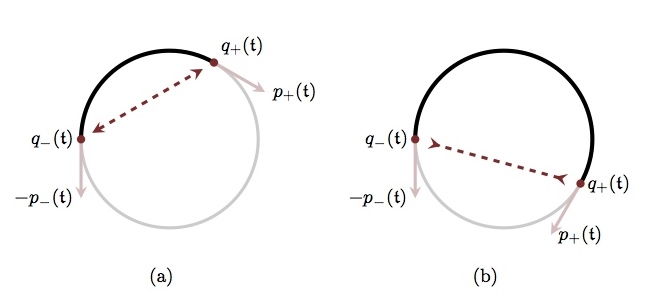
\includegraphics[scale=0.5]{cropped_nuts_image}

Even though the No-U-Turn sampler is named after its termination criterion, which can be described broadly as terminating whenever the trajectory starts to make a u-turn, the criterion itself is a rather crude heuristics that is not justified by any theory. The main advance of the paper is the devise of a correct and efficient way to construct dynamic leapfrog trajectories by recursively building binary trees. The termination criterion can be further improved, and STAN indeed adopts NUTS criteria more general than the original and others where the u-turn aspect is done away with. 

First we look further into the No-U-Turn termination criterion. From linear algebra, we know that $x^Ty > 0 $ can be interpreted to say that those two vectors form an acute angle. Then the No-U-Turn criterion 
\begin{align*}
&p_{+}^T (q_+ -q_-) < 0 \Leftrightarrow p_+^T (q_- - q_+) > 0 \\
&p_{-}^T (q_+ -q_-) < 0 \Leftrightarrow -p_-^T (q_+ - q_-) > 0 \\
\end{align*}
can be explained visually by figures (a) and (b). Figure (a) shows when the trajectory does not satisfy the terminating criterion and expansion continues. Figure (b) shows when the criterion is satisfied and expansion stops. This idea is generalized in \cite{betancourt2013generalizing}, where the dot product 
\begin{align*}
 p_{+}^T (q_{+} -q_{-})  
 &=p_{+}^T \int_{t=0}^{T} M^{-1}p(t) dt   \\
 &=p_{+}^T M^{-1} \int_{t=0}^{T} p(t)dt \\
 &=(M^{-1} p_{+})^T  \int_{t=0}^{T} p(t)dt \\
 &= p^{\#}_{+}  \int_{t=0}^{T} p(t)dt \\
 &\approx p^{\#}_{+} \sum_{i=0}^n p(t_{k_i}) \\
 &=  p^{\#}_{+} \sum_{z \sim \mathbf{t}} p(z) \\
\end{align*} 
is rewritten to accommodate variations of the HMC sampler where matrices other than the identity are set as the mass matrix. It is in fact the version of the terminating criterion implemented currently in STAN. Note that in this implementation the criterion is no longer dependent on the position variables $q$. The algorithm for this version of NUTS needs to be adjusted slightly to include a term accumulating the sum of $p$ variables across the subtrees. Pseudocode is provided below.
\begin{algorithm}
  	\DontPrintSemicolon
	\SetKwFunction{FBuildTree}{G-BuildTree}

    \KwIn{initial position $q_0$, step size $\epsilon$, joint density $\pi$} 
    Re-sample $p_0 \sim \mathcal{N}(0,\mathbb{I})$ \;
    Initialize $q_{-} = q_0 , q_{+} = q_0 , p_{-} =p_0 , p_+ = p_0, p_+^{\#} = M^{-1}p_+,p_-^{\#} = M^{-1}p_-, p_s = p_0, j =0 ,	q_{\text{next}} = q_0 , s = 1 , w = \pi(q_0,p_0)$ \;
    \While{$s=1$}{
    Choose a direction $v_j \sim \text{Uniform}(\{-1,1\}) $ \;
    \eIf{$v_j = -1$}{
    		$q_-,p_-,-,-,q',s',w',p_{s'} \leftarrow \text{G-BuildTree}(q_-,p_-,v_j,j,\epsilon)$\;
    }{
    		$-,-,q_+,p_+,q',s',w',p_{s'} \leftarrow \text{G-BuildTree}(q_+,p_+,v_j,j,\epsilon)$\;
    }
    \If{$s'=\text{True}$}{
    		With probability $\min(1,\frac{w'}{w})$, set $q_{\text{next}} \leftarrow q_-$\;
    		$p_{s} = p_{s} + p_{s'} $\;
    		$p_+^\# \leftarrow M^{-1} p_{+} $\;
		$p_-^\# \leftarrow M^{-1} p_{-} $\;
    		
    		
    }
    $ w = w + w'$\;
    $ s = s' \mathbb{I}[(q_+ - q_-) \cdot p_-^\# \ge 0 ] \mathbb{I}[(q_+ - q_-) \cdot p_+^\#  \ge 0 ] $\;
    $j = j+1 $ \;
    
    }

\KwRet{$q_{\text{next}}$}

\FBuildTree{$q, p, v, j, \epsilon$}{\;
        \eIf{$j=0$}{
Base case: take one step in direction $v$ \;
$ q' , p' \leftarrow \text{Leapfrog}(q,p,v\epsilon) $ \;
$ w' \leftarrow \pi(q',p') $ \;
$s' = \text{True}$ \;
\KwRet{$q',p',q',p',q',s',w',p_{s'}$} \;

}{
	$p_s = 0 $\;
	$q_-,p_-,q_+,p_+,q',s',w',p_{s'} \leftarrow \text{G-BuildTree}(q,p,v,j-1,\epsilon) $ \;
	
	\If{$s'=\text{True}$}{
		$p_s = p_s + p_{s'}$\;
		\eIf{$v=-1$}{
			$q_-,p_-,-,-,q'',s'',w'',p_{s''} \leftarrow \text{G-BuildTree}(q_-,p_-,v,j-1,\epsilon)$ \;
		}{
			$-,-,q_+,p_+,q'',s'',w'',p_{s''} \leftarrow \text{G-BuildTree}(q_+,p_+,v,j-1,\epsilon)$ \;
		}
		\If{$s''=\text{True}$}{
		
		With probability $\min(1, \frac{w''}{w'+w''})$ , set $q' = q''$. \;
		$p_+^\# \leftarrow M^{-1} p_{+} $\;
		$p_-^\# \leftarrow M^{-1} p_{-} $\;
		$ s' \leftarrow s'' \mathbb{I}[(q_+ - q_- )\cdot p_-^\# \ge 0 ] \mathbb{I}[(q_+ - q_- )\cdot p_+^\# \ge 0 ]$ \;
		$w' \leftarrow w' + w'' $ \;
		$p_{s} = p_{s} + p_{s''} $\;
		
		}
	}
	\KwRet{$q_-,p_-,q_+,p_+,q',s',w',p_{s'}$}\;
}
    }
\caption{Generalized No U-Turn Sampler Update}
\end{algorithm}


The Exhaustive Hamiltonian Monte Carlo (XHMC) termination criterion  relies on a significant amount of differential geometry for its justification. For example one can easily finds parts of the paper that read "an exhaustion ,$T_{\delta}(z)$, is the family of integration times in the contangent bundle such that the temporal change of the virial along the resulting Hamiltonian flow is uniformly bounded". Understanding fully the mathematics behind it is beyond the scope of this thesis. From my understanding it is a proxy to to monitor the return of a leapfrog trajectory to a neighbourhood around its initial point after having explored the energy level set. With a smaller threshold meant to push the neighbourhood smaller, hence forcing the exploration to continue for longer. Luckily the numerical quantities that needs to be computed are quite easily understood. In the original paper \cite{betancourt2016identifying}, the author showed improved sampling over the NUTS criterion as indicated by increased effective sample size on correlated distributions. 

The exhaustive termination criterion is defined as follows: given a threshold $\delta > 0$, terminates expansion of the trajectory when 
\[  \Bigl |\frac{1}{|\mathbf{t}|} \sum_{z \in \mathbf{t}} \mathbb{P}[z | \mathbf{t}] \frac{dG}{dt}(z) \Bigr | < \delta, \]
where 
\[ \mathbb{P}[z| \mathbf{t}] = \frac{\exp^{-H(z)}}{\sum_{z' \in \mathbf{t}} \exp^{-H(z')}}. \]
The sum can be interpreted as a numerical approximation of an integration over the Hamiltonian flow $\phi_{t}^H(z)$

\[ \lim_{|\mathbf{t}| \rightarrow \infty} \frac{1}{|\mathbf{t}|} \sum_{z \in \mathbf{t}} \mathbb{P}[z | \mathbf{t}] \frac{dG}{dt}(z)  = \lim_{\mathcal{T} \rightarrow \infty} \frac{1}{\mathcal{T}} \int_0^\mathcal{T} dt \frac{dG}{dt} \circ \phi_{t}^H(z) = 0. \]

For HMC samplers the virial can be simplified as follows:
\begin{align*}
 \frac{dG}{dt} &= \frac{d}{dt}\sum_{i=1}^D q_i p_i \\
 &= \sum_{i=1}^D p_i \frac{dq_i}{dt} + q_i \frac{dp_i}{dt} \\
 &= \sum_{i=1}^D [M^{-1}p]_i p_i - q_i \frac{\partial V}{\partial q_i} \\
 &= 2 T(p) - q \cdot \frac{\partial V}{\partial q}.\\
\end{align*}

\begin{algorithm}
  	\DontPrintSemicolon
	\SetKwFunction{FBuildTree}{XHMC-BuildTree}

    \KwIn{initial position $q_0$, step size $\epsilon$, joint density $\pi$} 
    Re-sample $p_0 \sim \mathcal{N}(0,\mathbb{I})$ \;
    Initialize $q_{-} = q_0 , q_{+} = q_0 , p_{-} =p_0 , p_+ = p_0, j =0 ,	q_{\text{next}} = q_0 , s = 1 , w = \pi(q_0,p_0), {ave} = \frac{dG}{dt}(q_0,p_0)$ \;
    \While{$s=1$}{
    Choose a direction $v_j \sim \text{Uniform}(-1,1) $ \;
    \eIf{$v_j = -1$}{
    		$q_-,p_-,-,-,q',s',w',{ave}' \leftarrow \text{XHMC-BuildTree}(q_-,p_-,v_j,j,\epsilon)$\;
    }{
    		$-,-,q_+,p_+,q',s',w',{ave}' \leftarrow \text{XHMC-BuildTree}(q_+,p_+,v_j,j,\epsilon)$\;
    }
    \If{$s'=1$}{
    		With probability $\min(1,\frac{w'}{w})$, set $q_{\text{next}} \leftarrow q_-$\;
    }
     Update ${ave}$ by incorporating ${ave}' $\;
    $ w = w + w'$\;
    $ s = s \mathbb{I}[ \frac{1}{2^j} |{ave} | \ge \delta ] $\;
    $j = j+1 $ \;
    
    }

\KwRet{$q_{\text{next}}$}

\FBuildTree{$q, p, v, j, \epsilon$}{\;
        \eIf{$j=0$}{
Base case: take one step in direction $v$ \;
$ q' , p' \leftarrow \text{Leapfrog}(q,p,v\epsilon) $ \;
$ w' \leftarrow \pi(q',p') $ \;
$ {ave}' \leftarrow \frac{dG}{dt}(q',p') $\;
\KwRet{$q_-,p_-,q_+,p_+,q',s',w',{ave}'$} \;

}{
	$q_-,p_-,q_+,p_+,q',s',w',{ave}' \leftarrow \text{XHMC-BuildTree}(q,p,v,j-1,\epsilon) $ \;
	
	\If{$s'=1$}{
		\eIf{$v=-1$}{
			$q_-,p_-,-,-,q'',s'',w'',ave'' \leftarrow \text{XHMC-BuildTree}(q_-,p_-,v,j-1,\epsilon)$ \;
		}{
			$-,-,q_+,p_+,q'',s'',w'',{ave}'' \leftarrow \text{XHMC-BuildTree}(q_+,p_+,v,j-1,\epsilon)$ \;
		}
		With probability $\min(1, \frac{w''}{w'+w''})$ , set $q' = q''$. \;
		Update $ave$ by incorporating $w'$ and ${ave}'$ \;
		$ s' \leftarrow s''  \mathbb{I}[ \frac{1}{2^j} |{ave} | \ge \delta ] $ \;
		$w' \leftarrow w' + w'' $ \;
	}
\KwRet{$q_{-},p_{-},q_{+},p_{+},q',s',w',{ave}'$}\;
}
    }
\caption{Exhaustive Hamiltonian Monte Carlo Sampler Update}
\end{algorithm}


\section{Adaptive Tuning of Step Size}


For one dimensional potential energy function $V(q) = \frac{q^2}{2\sigma^2}$,
that is, normal distributed with variance $\sigma^2$. Writing out the matrix that encodes the linear mapping from $(q(t),p(t))$ to $(q(t+\epsilon),p(t+\epsilon))$ gives that the mapping is stable if $\epsilon < 2 \sigma$, and diverges otherwise. 

For a general multivariate $q$ with arbitrary potential energy function, equivalent to a general density function, we can approximate the potential energy function with a second order Taylor expansion, so that the $q^2$ term in the Taylor expansion of $V(q)$ has coefficient $\frac{1}{2} \frac{\partial^2 V}{\partial q^2}$  
By matching the two expressions we get 
\[ \sigma \approx ( \frac{\partial^2 V}{\partial q^2})^{-1/2} \]

So by setting $\epsilon$ to that value, we are exactly in the middle of the domain of allowable step sizes, equivalent to half of the boundary limit. While this is a useful heuristic to help one thinks about setting the stepsize,
care has to be taken to evaluate the second derivative using values of the current parameters, because then the leapfrog steps are no longer reversible; that is since the stepsize is position dependent, we would get different step sizes at different ends of a trajectory, so when we reverse direction at the other end the trajectory might not be able return to the starting point. This heuristic has been used to guide step size selection in Neal's work on Bayesian neural networks with hierarchical priors.


Now, we describe how the step size is automatically tuned in STAN. First, keep
in mind that the step size is adapted only during the warm-up phase and stays
fixed during the sampling phase. This ensures the correctness of the algorithm
as the induced Markov chain resulted from an adaptive step size may not be
reversible. One way of manual tuning is try to find the step size
$\epsilon'$ that would result in an acceptance probability of $0.65$. The
acceptance probability is an average quantity, calculated as an expectation
over a chain. That is, we try to optimize $\epsilon \in \mathbb{R}$ with respect
to the function 
\[ h(\epsilon) = E_\pi[f(X)|\epsilon]  = \lim_{T \rightarrow \infty} \frac{1}{T}
\sum_{t=1}^T E[f(X_t)|\epsilon] \]

where $f(X_t)$ denotes the acceptance probability for iteration $t$. The
second equality comes from the convergence of the MCMC sampler. This is a
stochastic optimization problem, and STAN uses the dual averaging scheme of
Nesterov  to adapt the step size. The dual averaging scheme works in general as
follows. Suppose we are trying to find $x\in \mathbb{R}$ such that $h(x) =
E[H_t|x] = 0$ then we perform the updates 

\[x_{t+1}  = \mu - \frac{\sqrt{t}}{\gamma} \frac{1}{t+t_0} \sum_{i=1}^tH_i;
\bar{x}_{t+1} = \eta_t x_{t+1} + (1-\eta_t) \bar{x}_t \]

where $\mu$ is the target that the $x_t$'s are shrunk towards, $\gamma > 0$ a
parameter that controls the amount of shrinkage, $t_0 \ge 0$ a parameter that
stabilizes the early iterations, and $\eta_t = t^{-\kappa},\kappa>0$ is a
step size schedule ensuring convergence. Since $\epsilon>0$, this is technically
a constrained optimization problem, but it can be easily converted into an
unconstrained problem by optimizing for $\log(\epsilon)$ instead. 

\begin{algorithm}
\KwIn{Target Metropolis acceptance rate $\delta$, initial step size $\epsilon_0$, duration of tuning $M^{adapt}$ }

Initialize $\overline{H}_0 = 0, \gamma = 0.05, t_0 = 10 ,\kappa = 0.8 , \mu = \log(10\epsilon_0)$ \;
	
	Calculate acceptance rate $\alpha$ using $\epsilon_0$. \;
\For{$m = 1:M^{adapt}$}{
	 $\overline{H}_m = (1- \frac{1}{m+t_0}) \overline{H}_{m-1} + \frac{1}{m + t_0} (\delta - \alpha) $ \;
	 $\log \epsilon_m = \mu - \frac{\sqrt{m}}{\gamma} \overline{H}_m $ \;
	 $\log \overline{\epsilon}_m = m^{-\kappa} \log \epsilon_m + (1-m^{-\kappa}) \log \overline{\epsilon}_{m-1} $ \;
	
	Update acceptance rate $\alpha$ using $\overline{\epsilon}_m$ \;
	
}

\caption{dual averaging tuning of $\epsilon$ }
\end{algorithm}

Even with the dual averaging algorithm for adaptive tuning of the step size, it is still an optimization that requires an initialization. In Stan the original doubling-halving heuristic for initializing the dual averaging optimizer is used. It works by repeatedly doubling or halving the step size, integrating the system for one leapfrog step and evaluating the acceptance rate, until the rate crosses the 50 \% threshold. Hence it avoids starting off with a too large or small step size. 
\begin{algorithm}
Initialize $\epsilon = 1$, momentum $p \sim \mathcal{N}(0,\mathbb{I}) $ \;
$(q',p') \leftarrow \text{Leapfrog}(q,p,\epsilon) $ \;
$a \leftarrow 2 \mathbb{I}[ \frac{\pi(q',p')}{\pi(q,p)} > 0.5 ] -1 $\;
\While{ $(\frac{\pi(q',p')}{\pi(q,p)} )^a > 2^{-a} $}{
	$\epsilon \leftarrow 2^a \epsilon$ \;
	$(q',p') \leftarrow \text{Leapfrog}(q,p,\epsilon) $ \;
}
\KwRet{$\epsilon$}
\caption{find initial $\epsilon$} 
\end{algorithm}

\section{Adaptive Tuning of HMC Metric}
Stan divides the tuning period into a number of windows of different lengths. The following quantities,followed by their current default values in brackets, are of relevance in this discussion: 

\begin{enumerate}
\item Initial buffer (n=75): the first window of the sampling stage, where only the step size parameter is updated by dual averaging .

\item End buffer (n=50): the last window of the sampling stage, where the covariance metric is fixed and only the step size is updated and allows it to stabilize.

\item Window size (n=25): the base length of interval for updating the covariance metric. 
\end{enumerate}

Both the step size and covariance metric are updated during the tuning stage. And it proceeds as follows: the covariance metric is initialized by the identity matrix and an initial step size found by the doubling-halving heuristic. Parameter tuning happens in three stages. The first is the initial buffer, where only $\epsilon $ is updated. In the second stage, both the step size and covariance metric are updated. While $\epsilon$ is updated after every MCMC transition, because the dual averaging procedure only requires an acceptance rate, the covariance metric is updated only after the number of MCMC samples collected equals the current window size. Then compute the empirical covariance and set the metric to its inverse. Then double the window size or increase it to cover the rest of the remaining second stage if doubling is impossible. The third and last stage, which is the end buffer, updates the step size only. 

The algorithm is designed so that the covariance metric is not updated immediately at the start of the tuning stage, because the model might be initialized particularly poorly and hence the initial examples could be misleading. The doubling of window sizes is to allow progressive improvement of the covariance metric. For larger window sizes, the memory requirement for storing all the MCMC samples to estimate the covariance matrix could be prohibitive. Therefore, STAN actually uses an online algorithm for calculating the covariance, whose memory complexity is independent of the window size, which we will discuss in a later section.

\section{HMC-Specific Sampling Diagnostics}
bfmi , divergence ( talk about example 8 school) , tree depth ,

First we describe how Stan uses
divergence to diagnose $\epsilon$'s that are too large. A large constant
is selected, say $Th = 1000$, then after each proposal $(q_i,p_i)$, we compare the
energy value $H(q_i,p_i)$ with that of the previous state $H(q_{i-1},p_{i-1})$,
if $|H(q_i,p_i) - H(q_{i-1},p_{i-1})|> Th$ then a divergence is flagged and the
proposal rejected. This necessarily slows down the the sampler and increases the overall correlation between successive samples. But a divergence should not be interpreted as simply a rejected proposal. The presence of a divergence should call into question the correctness of the samples; the sample
drawn may be biased and hence invalid.
 At the end of the sampling stage, the total number of
divergence indicates potential problem with the chosen step size. Typically the
only response available is to reduce the step size and slow down sampling.
If the problem persists, it may call for reparametrization as the parameter
space may have many sharp edges and steep wells that no step sizes are small
enough to navigate the space.  This is not a diagnostic to be ignored. The recommended practice is zero tolerance for divergent transitions. Even a low number (say $\le 5 $ ) can cause biased samples.

In a static sampler we only need to check for divergence at the end of the leapfrog trajectory. For a NUTS sampler, since each state in the trajectory is considered for acceptance when it is first generated, that means we need to check for divergence for each of them. 


The second diagnostic tool that comes with Stan is the Bayesian fraction of
missing information (BFMI). It detects a mismatched conditional Hamiltonian
energy function
distribution when compared to the marginal Hamiltonian distribution. 

In a HMC sampler, the leapfrog step is a deterministic process
restricted to exploring a level set determined by the 
initial positions $(q_i,p_i)$ at the start of the trajectory. Given the previous 
state $q_i$, the only randomness introduced in the sampling process comes from the resampling of the auxiliary
momentum distribution.  The BFMI it is defined as 
\[ \text{BFMI} = \frac{ E_\pi[Var_{\pi_{H|q}}[H|q]]}{Var_{\pi_H}[H]} \]
where $\pi$ is the marginal distribution of $q$ and $\pi_{H|q}$ and $\pi_{H}$
are the conditional and marginal distributions of the Hamiltonian energy
function $H$ respectively.Since the goal is
to explore the energy parameter space , we want the two energy distributions, 
closely match each other. BFMI allows us to measure that match.

 In practice the expectations must be estimated, but
it is easily done by evaluating the energy function at the values from the
generated Markov chain. Suppose $N+1$ samples are drawn, the estimated BFMI 

\[ \text{E-BFMI} = \frac{\sum_{n=1}^N(H_n-H_{n-1})^2}{\sum_{n=0}(H_n-\bar{H})^2} \]
where $H_n = H(q_n,p_n)$ and $\overline{H}=\frac{1}{N+1}\sum_{n=0}^N H_n$. From basic
probability we have $0 \le BFMI \le 1 $ and the optimal value is when it is
1. A low value of $\text{E-BFMI}$ suggests that the auxiliary momentum distribution is
inefficient for sampling. 

 
\section{Other Sampling Diagnostics}

Other than divergence and BFMI, Stan also includes MCMC convergence diagnostics that are not specific to HMC samplers. They are the potential scale reduction factor and effective sample size. In the discussion that follows we assume the parameter under investigation is a one dimensional real variable $\psi$, it can be the log-posterior, the variance parameter for a regression model with normal prior, or the posterior mean of a covariate of interest.


The Potential scale reduction factor, also commonly referred to as R hat $\hat{R}$ , can be thought of as the factor by which the scale of the current distribution for $\psi$ might be reduced if the simulations were continued in the limit $n \rightarrow \infty$. This quantity should converge to $1$ as $n \rightarrow \infty$. If $\hat{R}$ is high, $ > 1.1 $, for example, we might we want to continue simulation. 

It is defined as follows. Suppose we have $m$ chains each of length $n$, where $\psi_{ij}$ is the $i$th term in chain $j$. Then we have 

\begin{align*}
&B = \frac{n}{m-1} \sum_{j=1}^{m}(\overline{\psi}_{\cdot j} - \overline{\psi}_{\cdot \cdot})^2, \text{ where } 
\overline{\psi}_{\cdot j} = \frac{1}{n} \sum_{i=1}^n \psi_{ij} , \overline{\psi}_{\cdot \cdot} = \frac{1}{m} \sum_{j=1}^m \overline{\psi}_{\cdot j }
 \\
&W = \frac{1}{m} \sum_{j=1}^m s_j^2 , \text{ where }
s_j^2 = \frac{1}{n-1} \sum_{i=1}^n (\psi_{ij} - \overline{\psi}_{\cdot j } )^2.\\
& \hat{\text{var}}^+(\psi|y) = \frac{n-1}{n} W + \frac{1}{n} B \\
& \hat{R} = \sqrt{\frac{\hat{\text{var}}^+(\psi|y)}{W}}. \\
\end{align*}
The Effective Sample Size (ESS) takes into account the autocorrelation inherent in MCMC samples and can be interpreted to represent the equivalent number of independent draws that a set of MCMC draws can replace, for example in calculating expectations and various posterior quantities. The ESS has been defined  differently in the literature (quote), the Stan implementation requires multiple chains and has the advantage that it mitigates the danger of overestimating the ESS when the chain has not converged. It is defined as 
\[n_{\text{eff}}  = \frac{mn}{1 + 2 \sum_{t=1}^\infty \rho_t}, \]

where  $\rho_t$ is the lag at time $t$. The variogram at $t$ 
\[V_t = \frac{1}{m(n-t)} \sum_{j=1}^m \sum_{i=t+1}^n (\psi_{i,j} - \psi_{i-t,j})^2 \]

and the fact $E[(\psi_i - \psi_{i-t})^2] = 2(1-\rho_t)\text{var}(\psi)$ helps to define an estimate for $lag$ at time $t$ 

\[\hat{\rho}_t = 1 - \frac{V_t}{2 \hat{\text{var}}^+}\]

Finally, the ess is estimated as 
\[\hat{n}_{\text{eff}} = \frac{mn}{1 + 2 \sum_{t=1}^T \hat{\rho}_t} \]

where $T$ is the first odd positive integer for which $\hat{\rho}_{T+1} + \hat{\rho}_{T+2} $ is negative. It is defined this way because it was observed that for large $T$ the estimates for the lags become too noisy. 
 
\section{Numeric tricks/Implementation tricks}

Below we list a number of numerical "tricks" that are nonetheless essential for a successful implementation of a HMC sampler, but is usually omitted in the literature. 

First, there is the logsumexp function, which enables numerical stable addition of probability functions on the log scale. While users of traditonal MCMC samplers like the Random Walk Metropolis Hastings should be familiar with the idea of computing the Hastings ratio on the log scale to avoid division of probabilities, the NUTS expansion requires updating the probability of the current state by adding the probability from the new subtree. So, instead of doing 
\[ w = w + w' \] 
we would instead have
\[ \log w = \text{logsumexp}(\log w, \log w' ). \]

\begin{algorithm}
\DontPrintSemicolon
\KwIn{$a,b$}
\KwOut{$c = \log(\exp(a)+ \exp(b)) $}
$s = \max(a,b) $\;
$c = s + \log( \exp(a-s) + \exp(b-s)) $\;

\KwRet{$c$}
\caption{logsumexp}
\end{algorithm}

Similarly, for the Exhaustive Hamiltonian Monte Carlo termination criterion a sum of $\frac{dG}{dt}$ weighted by the probability at the state need to calculated. A numerical stable method calculating both quantities is described below.

\begin{algorithm}
\DontPrintSemicolon
\KwIn{$a_1,\log w_1 , a_2, \log w_2$}
\KwOut{$a = \frac{a_1  w_1 + a_2 w_2}{w_1+w_2} ,\log w = \log (w_1 + w_2)$}

\eIf{$\log w_1 > \log w_2 $}{
	$e = \exp(\log w_1 - \log w_2 ) $\;
	$a = \frac{e \cdot a_1 + a_2}{1+e} $\;
	$\log w = \log w_2 + \log(1+e) $ \;
}{
	$e = \exp(\log w_2 - \log w_1 ) $\;
	$a = \frac{e \cdot a_2 + a_1}{1+e} $\;
	$\log w = \log w_1 + \log(1+e) $ \;
}
\KwRet{$a,\log w$}
\caption{Stable Sum }
\end{algorithm}

The pseudocode for numerically stble versions of generalized NUTS sampler (GNUTS) and XHMC are given below. Note that it also monitors divergence and rejects automatically any divergent transition.

\begin{algorithm}
	\SetKwFunction{BuildTree}{BuildTree}
	\DontPrintSemicolon

    \KwIn{initial position $q_0$, step size $\epsilon$, joint density $\pi$} 
    Re-sample $p_0 \sim \mathcal{N}(0,\mathbb{I})$ \;
    Initialize $q_{-} = q_0 , q_{+} = q_0 , p_{-} =p_0 , p_+ = p_0, j =0 ,	q_{\text{next}} = q_0 , s = 1 , \log w = H(q_0,p_0)$ \;
    \While{$s=1$}{
    Choose a direction $v_j \sim \text{Uniform}(\{-1,1\}) $ \;
    \eIf{$v_j = -1$}{
    		$q_-,p_-,-,-,q',s',\log w' \leftarrow \text{BuildTree}(q_-,p_-,v_j,j,\epsilon,\log w)$\;
    }{
    		$-,-,q_+,p_+,q',s',\log w' \leftarrow \text{BuildTree}(q_+,p_+,v_j,j,\epsilon,\log w)$\;
    }
    \If{$s'=1$}{
    		With probability $\text{exp}(\min(0,\log w' -\log w))$, set $q_{\text{next}} \leftarrow q_-$\;
    }
    $ w = \text{logsumexp}(w , w')$\;
    $ s = s \mathbb{I}[(q_+ - q_-) \cdot p_- \ge 0 ] \mathbb{I}[(q_+ - q_-) \cdot p_+ \ge 0 ] $\;
    $j = j+1 $ \;
    
    }

\KwRet{$q_{\text{next}}$}\;
\BuildTree{initial position $q$, initial momentum $p$,integration direction $v$,tree depth $j$,step size $\epsilon$,initial Hamiltonian $H_0$} \;
\eIf{$j=0$}{
Base case: take one step in direction $v$ \;
$ q' , p' \leftarrow \text{Leapfrog}(q,p,v\epsilon,H_0) $ \;
$ \log w' \leftarrow H(q',p') $ \;
$ s' = \text{True} \text{ and } \mathbb{I}[\log w' - H_0 > 1000] $\;
\KwRet{$q_-,p_-,q_+,p_+,q',s',\log w'$} \;

}{
	$q_-,p_-,q_+,p_+,q',s',\log w' \leftarrow \text{BuildTree}(q,p,v,j-1,\epsilon,H_0) $ \;
	
	\If{$s'=1$}{
		\eIf{$v=-1$}{
			$q_-,p_-,-,-,q'',s'',w'' \leftarrow \text{BuildTree}(q_-,p_-,v,j-1,\epsilon,H_0)$ \;
		}{
			$-,-,q_+,p_+,q'',s'',w'' \leftarrow \text{BuildTree}(q_+,p_+,v,j-1,\epsilon,H_0)$ \;
		}
		With probability $\text{exp}(\min(0, \log{w''}-\text{logsumexp}(w',w'')))$ , set $q' = p''$. \;
		$ s' \leftarrow s'' \mathbb{I}[(q_+ - q_- )\cdot p^- \ge 0 ] \mathbb{I}[(q_+ - q_- )\cdot p_+ \ge 0 ]$ \;
		$\log w' \leftarrow \text{logsumexp}(w', w'') $ \;
	}
	\KwRet{$q_-,p_-,q_+,p_+,q',s',\log w' $ }\;
}
\caption{Numerically stable No U-Turn Sampler Update with Unity Covariance Metric }
\end{algorithm}

\begin{algorithm}
  	\DontPrintSemicolon
	\SetKwFunction{FBuildTree}{XHMC-BuildTree}

    \KwIn{initial position $q_0$, step size $\epsilon$, energy function $H$} 
    Re-sample $p_0 \sim \mathcal{N}(0,\mathbb{I})$ \;
    Initialize $q_{-} = q_0 , q_{+} = q_0 , p_{-} =p_0 , p_+ = p_0, j =0 ,	q_{\text{next}} = q_0 , s = 1 , \log w = H(q_0,p_0), {ave} = \frac{dG}{dt}(q_0,p_0)$ \;
    \While{$s=1$}{
    Choose a direction $v_j \sim \text{Uniform}(-1,1) $ \;
    \eIf{$v_j = -1$}{
    		$q_-,p_-,-,-,q',s',\log w',{ave}' \leftarrow \text{XHMC-BuildTree}(q_-,p_-,v_j,j,\epsilon,\log w )$\;
    }{
    		$-,-,q_+,p_+,q',s',\log w',{ave}' \leftarrow \text{XHMC-BuildTree}(q_+,p_+,v_j,j,\epsilon,\log w)$\;
    }
    \If{$s'=1$}{
    		With probability $\text{exp}(\min(0,\log w'-\log w)$, set $q_{\text{next}} \leftarrow q_-$\;
    }
     Update ${ave}$ by incorporating ${ave}' $\;
    $ ave, \log w  = \text{stablesum}(ave,\log w,ave',\log w')$\;
    $ s = s \mathbb{I}[ \frac{1}{2^j} |{ave} | \ge \delta ] $\;
    $j = j+1 $ \;
    }
\KwRet{$q_{\text{next}}$}\;

\FBuildTree{$q, p, v, j, \epsilon,H_0$}{\;
        \eIf{$j=0$}{
Base case: take one step in direction $v$ \;
$ q' , p' \leftarrow \text{Leapfrog}(q,p,v\epsilon) $ \;
$ \log w' \leftarrow H(q',p') $ \;
$ {ave}' \leftarrow \frac{dG}{dt}(q',p') $\;
$ s' = \text{True} \text{ and } \mathbb{I}[\log w' - H_0 > 1000] $\;
\KwRet{$q_-,p_-,q_+,p_+,q',s',\log w',{ave}'$} \;

}{
	$q_-,p_-,q_+,p_+,q',s',\log w',{ave}' \leftarrow \text{XHMC-BuildTree}(q,p,v,j-1,\epsilon,H_0) $ \;
	
	\If{$s'=1$}{
		\eIf{$v=-1$}{
			$q_-,p_-,-,-,q'',s'',\log w'',ave'' \leftarrow \text{XHMC-BuildTree}(q_-,p_-,v,j-1,\epsilon,H_0)$ \;
		}{
			$-,-,q_+,p_+,q'',s'',\log w'',{ave}'' \leftarrow \text{XHMC-BuildTree}(q_+,p_+,v,j-1,\epsilon,H_0)$ \;
		}
		With probability $\text{exp}(\min(0, \log w'' -\text{logsumexp}(w',w''))$ , set $q' = q''$. \;
		$ave,\log w \leftarrow \text{stablesum}(ave,\log w,ave',\log w')$ \;
		$ s' \leftarrow s''  \mathbb{I}[ \frac{1}{2^j} |{ave} | \ge \delta ] $ \;
	}
\KwRet{$q_{-},p_{-},q_{+},p_{+},q',s',\log w',{ave}'$}\;
}
}
\caption{Numerically stable Exhaustive Hamiltonian Monte Carlo Sampler Update}
\end{algorithm}




Next we show the online algorithm used by Stan to calculate the empirical covariance matrix of the target distribution during the tuning stage. It uses the Welford algorithm, which only requires storing one vector of the same size as the mean and one matrix of the same dimension as the covariance. 
\begin{algorithm}
\DontPrintSemicolon
\KwIn{current sample counter $t$,accumulator for the mean $m$, accumulator for covariance $m_2$, current sample $x$}

$\delta = x-m$ \;
$m = m + \frac{\delta}{t} $\;
$m_2 = (x-m)\delta^T $ \;
$\mu = m $\;
$\Sigma = \frac{m_2}{t-1} $\;
\KwRet{$m,m_2,\mu,\Sigma$}
\caption{Welford algorithm}
\end{algorithm}

Since HMC only works on unconstrained parameter spaces, any constrained parameters, for example the variance need to be transformed into unconstrained variables, and transformed back into the original form after the leapfrog steps to calculate acceptance rate. The following identities are useful for coding up the distributions for sampling by HMC.

Suppose $y \ge 0 $ is the original parameter. Then it is first transformed
 \[ X = \text{exp}(y)  \]
 
 and the log posterior is adjusted by a Jacobian term.
\begin{align*}
p_Y(y) = p_X(f^{-1}(y)) \ |\frac{d}{dY} f^{-1}(y) |\\
p_Y(y) = p_X(\exp(y)) \cdot \exp(y) \\
\log p_Y(y) = \log p_X(\exp(y)) + y \\
\end{align*}
When calculating the ESS, the variogram $V_t$ involves a summation term of the form $\sum_{n=t+1}^N (\theta_{n} - \theta_{n-t})^2$, which can be time-consuming when carried by brtute force. From discrete mathematics we know that the Fast Fourrier Transform (FFT) can be used to speed up calculation for sums of the form 

\[ \sum_{n=t+1}^N \theta_n \theta_{n-t}.  \]

We can rewrite the sum into a linear combination of the desired form:

\begin{align*}
 \sum_{n=t+1}^N (\theta_{n} - \theta_{n-t})^2 &= \sum_{n=t+1}^N \theta_n^2 - 2 \theta_n \theta_{n-t} + \theta_{n-t}^2  \\
 &= \sum_{n=t+1}^N \theta_n^2 -2 \sum_{n=t+1}^N \theta_n \theta_{n-t} + \sum_{n=t+1}^N \theta_{n-t}^2 \\ 
  &= \sum_{n=t+1}^N  \theta_n^2 \cdot 1  -2 \sum_{n=t+1}^N \theta_n \theta_{n-t} + \sum_{n=t+1}^N 1 \cdot \theta_{n-t}^2 \\
\end{align*}
Finally we discuss a useful heuristics for debugging MCMC samplers. Suppose we have coded a sampler and it seems to run smoothly without a hitch, one might want to use it to sample from a distribution with known mean and covariance, and see if the MCMC samples converge to them in the first and second moments. However, since the empirical mean and covariance will never match exactly the true values, how should we decide if the estimates are close enoguh?


As an example, suppose we want to sample from a bivariate normal distribution with known mean and covariance matrix. Say $\mathcal{N}(\mu,\Sigma) $, where 

\begin{displaymath}
\mathlarger{\Sigma} = 
\begin{bmatrix}
\sigma^2_1 &\sigma_{12}^2 \\
\sigma_{21}^2 &\sigma^2_2 \\
\end{bmatrix}.
\end{displaymath}

Given a chain of $n$ MCMC samples $\{x_i\}_{i=1:n}$ generated by the sampler to be tested, we could estimate  the target mean by $ \frac{1}{n-1} \sum_{i=1}^ n x_i$. Since $E[X-\mu] = 0$, we would expect the generated quantity $\eta= \frac{1}{n-1} \sum_{i=1}^ n x_i -\mu$ to decrease with increasing number of samples. We could monitor $\eta$ by comparing it with its Monte Carlo standard error (MCSE) 

\[ \text{MCSE} = \frac{\hat{\sigma}}{\sqrt{n_{\text{eff}}}} \]

where $\hat{\sigma}$ is the estimated standard deviation. By the Central Limit Theorem one would expect  $\eta \in (-\text{MCSE},\text{MCSE})$ with high probability.Similarly we can monitor quantities like $\frac{1}{n-1} \sum_{i=1}^n ({x_i}_1 -\mu_1)^2 - \sigma^2_1,  \frac{1}{n-1}^n \sum_{i=1}^n ({x_i}_1 - \mu_1)({x_i}_2 - \mu_2)^2 $ to assess convergence to the marginal variances and covariance.

One can then construct example models where the mean and covariance are known explicitly, simulate multiple chains and monitor quantities for approximate convergence, in the sense that the empirical estimated quantities differ from their exact quantities by a margin no larger than its MCSE (or its constant multiple .) 

The samplers implemented in this study have been tested on a two dimensional multivariate normal distribution with known covariance and Bayesian logistic regression problem whose posterior covariance is estimated by a long chain generated by Stan.

\chapter{Bayesian Neural Networks}
\section{Neal}

Deep Learning, a field in machine learning studying multilayered neural network models, has become quite successful in Artificial Intelligence tasks and a lot of research has been, and is being done to improve our understanding of these models and to apply them better and to more fields. See \cite{Goodfellow-et-al-2016-Book,lecun2015deep} for a general introduction into the methodology and application of deep learning, and \cite{schmidhuber2015deep} for an in-depth literature review. 

Before there was Deep Learning, a term which only came about in the mid 2000s, there were Neural Networks \cite{bishop1995neural,ripley2007pattern}, which were also hugely popular in the 90s, but eventually the enthusiasim for neural networks cooled off because they were perceived to be too computationally intensive and difficult to scale up. The main reason for this was the difficulty of training neural networks of more than one or two hidden layers. Traditional optimization techniques like stochastic gradient descent with backpropogation did not improve empirical test error for networks with more layers,not until ideas like pre-training to initialize optimization were experimented could we fit "deep" neural networks with more than 2 hidden layers. This rebooted the field, now rebranded as Deep Learning, and innovations like using the rectified linear units as activation functions \cite{nair2010rectified} to allow training deep networks without pre-training, and using GPUs to speed up the training process \cite{krizhevsky2012imagenet}, as well as the creation of software libraries like Theano \cite{bergstra2010theano}, Caffe \cite{jia2014caffe}, Tensorflow\cite{tensorflow2015-whitepaper}, and PyTorch \cite{paszke2017automatic}, just to name a few, that make building and training neural network models much easier by automating the backpropogation step with symbolic differentiation \cite{bahrampour2015comparative} and handles the transition between CPU and GPU computation modes. 

First we describe one of the most popular neural network models, the feedforward networks.

Suppose we have $n$ observed data points $\{y_i,x_i\}$ where $X_i \in
\mathcal{R}^p$ is a $p$-dimensional vector, then a feedforward neural network models the
data as follows:

\[y_i = \prod_{j=1}^Lg_j(V_jf_j(W_j))x_i \]
where $L$ is the number of layers of the network, $W_j$ a $n_j \times m_{j-1}$
weight matrix, $V_j$ a $m_j \times m_{j-1}$ weight matrix, and each $g_j$,$f_j$
a pair of activation functions that are usually non-linear functions. There are
usually no restrictions on what these activation functions must be other than on
$g_L$ which must match the data type of the $y_i$'s. For example, if $y_i$ are
binary observations then we would like the last output activate function to be a
logistic function so that it maps output to strictly $[0,1]$, just like in
logistic regression.

Popular activation functions in the classical neural network literature includes
the logistic function $f(x) = \frac{1}{1+\text{exp}(-x)} $ and the hyperbolic tangent function $h(x) =  2f(2x)-1$, but in modern deep
learning the Rectified linear unit (RELU) has come to dominate the field. It has
a simple form of $g(x)=\max{0,x}$, which is straightforward to do
backpropogation with despite a single point of nondifferentiability, and it was
found to improve optimization enormously. It's discovery has allowed training
neural network models with many more layers than 2 with random initialization of
weights, getting rid of the need for pre-training. 

While neural networks can have different numbers of layers and number of hidden
units within each layer, theoretically only one layer is sufficient to
approximate any function as we increase the number of hidden units \cite{hornik1991approximation}. 

For Bayesian neural networks where one puts a Gaussian prior distribution on the weights of model, it has been shown that for a one-hidden-layer model, the prior converges to a Gaussian process as the number of hidden units converge to infinity \cite{neal2012bayesian}.This gives a neat intrepretation of bayesian neural networks. 

Further work by \cite{gal2015dropout}, shows that heuristic training techniques such as dropout \cite{srivastava2014dropout}  are actually are actually doing variational inference with Deep Gaussian Process \cite{damianou2013deep} as its prior, a process where several GPs are stacked one after another. 

The most exact way to perform Bayesian inference for BNNs is still MCMC sampling as pioneered in Neal's thesis. In his work he put a conjugate hiearchical prior on the weights of the network and sampled the weights with HMC and the hyperparameter with block-Gibbs updates. One of his graduate students attempted to sample the weights and hyperparameters jointly with HMC but did not get better performance. Cho experimented with a Block Gibbs-HMC hybrid method where each conditional distribution is sampled alternatively by HMC. I experimented with a much simply alternative for joint sampling and found good results in terms of sample quality. 

For some theory on why, for the same number of hidden layers, it would be better to have multiple layers in a NN rather than a wide single-layer network, see \cite{montufar2014number}. 

Neal found that the windowed HMC sampler improves sampling in general, and also that evaluating the gradient using only a subset of the data would not deterioate performance significantly. We would seek to corroborate those observations in our own experiments.

When assessing convergence of the MCMC samples to the posterior distribution of a Bayesian neural network model, one needs to keep in mind that in general these models have a high number of local modes, usually as an exponential function of the number hidden units. \cite{bishop1995neural}. This means we cannot interpret the samples as being drawn from the full posterior distribution, but only from the neighbourhoods containing the local modes that the chains happen to settle around. That means looking at the potential scale reduction (Rhat) for individual weights is probably not that useful because it's not designed to handle multimodal distributions.  

It's still useful to monitor the convergence of the log posterior and of the E-BFMI statistics. Also it can still be useful to monitor the Rhat statistics for the hyperparameter if we can reasonably expect(as we can in the case for the variance parameter of a Bayesian neural network) it no to be multimodal. 



\section{Sampling for the Hyperparameter}

In Neal's work he separated the model parameters into groups, and put independent Gaussian-Inverse-Gamma priors on each of them. For example, let $W_{ij}$ let be the an entry in the weight matrix connecting the input covariates to the hidden units in the first layer. Then, the prior is 

\[W_{ij} \sim \mathcal{N}(0,\sigma^2), \sigma^{-2} \sim \text{Gamma}(a_0,b_0) \]

Assuming $n = |W|$, the  posterior distribution for the hyperparameter is once again Inverse-Gamma
\[\sigma^{-2}|W,X,y \sim \text{Gamma}(a_1,b_1)\]
\[a_1 = a_0 + \frac{1}{2} n  \]
\[b_1 = b_0 + \frac{1}{2} \sum_{ij} W_{ij}^2 \]

In Neal's work he alternated between sampling the lower-level weights with HMC and drawing from the conjugate posterior for the hyperparameter. The pseudocode is given below.
\begin{algorithm}
\KwIn{Initial variance $\sigma^2_0$, number of MCMC samples $M$}

\For{$ i = 1:M$ }{
	Sample $W_i \sim p(W|\sigma^2_{i-1},data)$ \;
	$a_1 = a_0 + \frac{1}{2} n $ \; 
	$b_1 = b_0 + \frac{1}{2} \sum_{ij} W_{ij}^2$ \;
	Update $\sigma^2 \sim \text{Inv-Gamma}(a_1,b_1)$ \;
}
\KwRet{$W_{i=1:M}$}
\caption{Blocks-Gibbs Sampler for NN weights and variance}
\end{algorithm}

In Cho's work, he experimented with joint sampling of the lower-level weights and hyperparameters. However, since the dual averaging scheme for automatic tuning the step size was not available at the time, he had to rely on the heuristics invented by Neal, which asks for alternate sampling of the conditional distributions in which the step size is dependent on the variables being held constant. He devised a scheme where the leapfrog steps in the joint parameter space have to be done separately for the two groups of parameters. 

A quick note on the parameterization used for the hierarchical prior. The non-centered parametrization is expected to mitigate the posterior correlation between the hyperparameter and the lower-level weights. Reducing posterior correlation is known to help improve sampling efficiency signficantly. 

We experimented with joint sampling under both parametrizations and found that non-centered parametrization is necessary for meaningful inference. The HMC also performs better than the Block-Gibbs sampler.

\section{SGHMC}
The idea of simulating Hamilotnian dynamics without the Metropolis acceptance step was first experimented in the statistics/machine learning literature by Neal \cite{neal1993bayesian} in a batch MCMC sampler for the posterior distribution of a BNN. He found that,with careful selection of the leapfrog step size, the biased samples achieve similar predictive performance as the full MCMC samples. Therefore, it seems to reason that for predictive tasks e.g. regression or classificaiton where observations are abundant, we could 
use a validation set (predictive performance) to select tuning parameters, hoping to trade off a bit of bias for better predictive performance. 

Another trick that helps to speed up the HMC sampler is data subsampling, also denoted partial gradient in Neal's thesis \cite{neal2012bayesian}.
Assuming there are $n$ data points, the potential energy function $V(q)$ can be written as 
\[ V(q) = -\log( \pi(q) \pi(q|data) = -\log(\pi(q)) -\log \pi(q|data) = -\log(\pi(q)) - \sum_{i=1}^n \log \pi(q|data_i) \]
where $\pi(q)$ is the prior density function and $\pi(q|data)$ is the likelihood function. Note that the finite series in the last expression above can be approximated as 
\[ \sum_{i=1}^n \log \pi(q|data_i) \approx \frac{n}{k} \sum_{i \in I} \log \pi(q|data_i) \]
where $I$ is a subset of $\{1,\dots, n\}$ of size $\frac{k}{n}$. 
More pratically, if we divide the datapoints into $M$ equally sized subsets. Then for any such subset $S$, the potential energy function can be approximated by 
\[ V(q) \approx    -\log(\pi(q)) + M \sum_{i \in S} \log(\pi(q|data_i)) = \tilde{V}(q) \] Data subsampling and omission of the Metropolis acceptance step are two key features of the stochastic gradient MCMC literature. In an overivew the stochastic gradient MCMC literature 
the authors summarized it as follows:
 "If the stationary distribution is not the target distribution, a Metropolis-Hastings (MH) correction can often be applied. Unfortunately, such correction steps require a costly computation on the entire
dataset. Even if one can compute the MH correction, if the dynamics do not nearly lead to the correct stationary distribution, then the rejection rate can be high even for short simulation periods h. Furthermore, for many stochastic gradient MCMC samplers, computing the probability of the reverse path is infeasible, obviating the use of MH. As such, a focus in the literature is on defining dynamics with the right target distribution, especially in large-data scenarios where MH corrections are computationally burdensome or infeasible.
"\cite{ma2015complete}

In Deep Learning, neural networks are usually fitted by stochastic gradient descent (SGD) \cite{ngiam2011optimization}.
This is a first order method like regular gradient descent \cite{wright1999numerical}, except at each weight update a random subset(batch) of datapoints are sampled to be the  observations, and the sequence of stepsizes over the optimiztion process must decay while satisfying the property

\[ \sum_{t=1}^\infty \epsilon_t = \infty , \sum_{t=1}^\infty \epsilon_t^2 < \infty \]

Theory from the stochastic optimization literature \cite{robbins1951stochastic} guarantees convergence to a local minimum. However, as per the norm in the optimization literature, the convergence property is usually only provable for easier classes of problems (.e.g. convex, quadratic functions) to which the likelihood of neural network models does not belong. Nonetheless, SGD has the advantage of easy implementation and low memory requirement ($O(D)$), and hence remains the predominant optimization method in deep learning.  

The success of SGD lies in being able to avoid evaluating the full likelihood, which has contribution from each data point, at each update. The problems that neural network models tend to be fitted are usually in the high-sample-size, high-dimensional regime, hence a full evaluation would slow down the algorithm significantly. A stochastic gradient extension to MCMC was first experimented by \cite{welling2011bayesian}, where the author proposed to use the following updates :

\[q_{t+1} = q_t + \frac{\epsilon_t}{2} ( \nabla \log p(q_t) + \frac{N}{n} \sum_{i \in \mathcal{D}} \nabla \log \pi(x_i|q_t) ) + \eta_t , \eta \sim \mathcal{N}(0,\epsilon_t) \]

where $\mathcal{D}$ is a random subset of $\{1,2, \dots, N\}$ of size $n$ sampled at each update of $q$. We assume there are $N$ observations in total. The step sizes are assumed to decay following the constraint stated above for SGD. The authors recommended setting $\epsilon_t = a(b+t)^{-\gamma} $ with $\gamma \in (0.5,1]$.  

The author proved that as the step sizes $\epsilon_t$ goes to $0$ the samples $\{q_t\}$ converge tothe Langevin dynamics targeting the posterior distribution. Of course, in practice we set lower bound on $\epsilon_t$ and stop decreasing the stepsize once it is small enough. Also, the fact the we are not doing the acceptance-rejection step means there will be a bias in our posterior samples, which unlike the samples drawn from a Metropolis-Hastings sampler, does not decrese to $0$ as we sample from the chain longer.


Simulating from the discrete approximation to a Langevin dynamics is the basis
for Langevin Monte Carlo (LMC) or Metropolis adjusted Langevin Algorithm (MALA), which
includes an acceptance-rejection step at each update. This can also be seen as a
special case of HMC where only one leapfrog step is used ($L=1$). It has been
demonstrated that HMC is much more efficient than LMC because it avoids random
walk. (Show $O(D^{4/3})$ vs $O(D^{5/4})$ kind of results). This inspires
Stochastic Gradient Hamilotian Monte Carlo (SGHMC), 
which extends HMC the way SGLD extends LMC. 



Applying MCMC methods to large datasets often involve 2 problems. First, evaluating the unnormalized posterior density
\[ \pi(D|q) = \prod_{i=1}^n \pi(x_i|q) \]
 is equivalent to passing through all datapoints, which alone can make the sampling algorithm unacceptably slow since all versions of the Metropolis-Hastings sampler requires such evaluations for proposing new samples. Second, models that require MCMC samples when a large number of datapoints are available are necessarily singular models. Using the terminology of \cite{watanabe2009algebraic}, regular models are models for which the bayesian central limit theorem \cite{le2012asymptotic} holds, that is, when the number of observations goes to infinity the posterior distribution of $q$ converges to a Normal distribution. Models that are non-regular are called singular models. A lot of methods designed to scale MCMC \cite{neiswanger2013asymptotically,scott2016bayes,} ultimately rely on this asymptotic normality for validity. Bayesian logistic regression is a classical model for which the CLT holds and is used in many papers to demonstrate the effectiveness of newly proposed large-scale MCMC methods. However, the very fact that asympotitic normality holds means there is little added utility to drawing MCMC samples from the posterior distribution, since a normal approximation would suffice. On the other hand, for singular models there is no guarantee that the estimates converge to the target posterior distribution. 

Asympotic normality is also assumed for the application of stochastic gradient mcmc methods to neural network models \cite{welling2011bayesian,chen2014stochastic,ahn2012bayesian,ding2014bayesian,ma2015complete}. Even though neural networks are singular models where the conditions for the central limit theorem do not hold, these methods have shown good predictive performance on a variety of datasets. This is opposite of what one would expect and merits further investigation.


Now we introduce the Stochastic gradient Hamiltonian Monte Carlo (SGHMC) \cite{chen2014stochastic}


\begin{algorithm}
    \caption{Stochastic Gradient HMC}
    \KwData{Input: $\eta,\hat{\beta},\epsilon,\alpha,n,M,L,q_0$}
        Initialize $\theta_0,v_0$ \;
        \For{$t = 1:M$}{
        $q^{0}=q_{t-1}$\;
        $v^{0} \sim \mathcal{N}(0,1) \times \epsilon $ \;
        
        \For{$i = 1:L$}{
        $q^{i} = q^{i-1} + v^{i-1}$ \;
        Sample $z \sim \mathcal{N}(0,2(\alpha-\hat{\beta} \eta))$ \;
        Sample minibatch and calculate $\nabla \tilde{V}(q)$  \;
        $v^{i} = -\eta \nabla \tilde{V}(q) - \alpha v^{i-1} + z$ \;
        }
        
        $q_t = q^{L}$ \;
        $v_t = v^{L}$ \;
        }
\end{algorithm}






Stochastic gradient Hamiltonian Monte Carlo \cite{chen2014stochastic}
relies on the assumption that the gradient of the log target density is normally distributed, which in turn comes from assuming independence of the observations $x$ and appealing to the central limit theorem.



\section{Priors}

The horseshoe prior was first proposed by quote as a Bayesian counterpart to the frequentist Lasso estimator in high-dimensional statistics. Like the lasso, it shrinks estimates for irrelevant covariates to zero. Compared to alternatives like the Bayesian Lasso \cite{park2008bayesian},  and the spike-and-slab prior \cite{mitchell1988bayesian}, it has the advantage of admitting full HMC sampling because it contains no discrete parameters.

It proceeds as follows: 
\[ \mathbf{\beta} = (\beta_1,\cdots,\beta_D)\]

\begin{align*}
 &\beta_j \sim \mathcal{N}(0,\tau^2\lambda^2) \\
 &\lambda_j \sim C^+(0,1),\, j = 1,\dots , D, \\
\end{align*}
where $C^+(0,1)$ is a half-Cauchy distribution with mean zero and variance one. The horseshoe prior is usually applied to regression problems where the number of samples were significantly fewer than the number of covariates and can be useful for models that require regularization, like neural networks \cite{ghosh2017model}.

However, the horseshoe prior sometimes causes divergent behaviour during sampling. The regularized horseshoe prior \cite{piironen2017sparsity} fixes this problem and is described below:

\begin{align*}
&\beta_j | \lambda_j, \tau, c \sim \mathcal{N}(0,\tau^2 \tilde{\lambda}_j^2) ,\, \tilde{\lambda}_j^2 = \frac{c^2 \lambda_j^2}{c^2 + \tau^2 \lambda_j^2} \\
&\lambda_j \sim C^+(0,1),\, j = 1,\dots,D\\
&c^2 \sim \text{Inv-Gamma}(2,8) .
\end{align*}
We note that the Cauchy distribution is equivalent to Student-t distribution of degree 1. A thick-tailed prior like the Student-t is known to cause divergent problems. Therefore, it is often written as a Normal-Inverse Gamma mixture to reduce posterior correlation. That is, $x \sim t_{\nu}(0,1) $ is 
equivalent to 
\begin{align*}
& x \sim \mathcal{N}(0,\sigma^2)\\
&\sigma^2 \sim \text{Inv-Gamma}(0.5,0.5). \\
\end{align*}
We can further reduce correlation by using a non-centered parametrization:
\begin{align*}
& x = z * \sigma \\
& z \sim \mathcal{N}^+(0,1)\\
&\sigma^2 \sim \text{Inv-Gamma}(0.5,0.5). \\
\end{align*}
The joint parameter space then becomes $(z,r_1^l,r_2^l,r_1^g,r_2^g) $,
where
\begin{align*}
& z \sim \mathcal{N}(0,1) \\
& \{r_1^l\}_j \sim \mathcal{N}^+(0,1) \, \forall j \\
& \{r_2^l\}_j \sim \text{Inv-Gamma}(0.5,0.5) \, \forall j  \\
& r_1^g \sim \mathcal{N}^+(0,1)  \\
& r_2^g \sim \text{Inv-Gamma}(0.5,0.5)   \\
& \lambda =  r_1^l \cdot r_2^l \\
& \tau = r_1^g \cdot r_2^g \\
& \beta = z \cdot \lambda \tau . \\
\end{align*}
Because the local and global $r_1$ parameters are constrained to be positive,the final unconstrained parameter space is $(z,\log r_1^l,r_2^l,\log r_1^g,r_2^g)$


Here we would briefly introduce the Automatic Relevance Determination (ARD) priors. It is a general way of assigning priors to the neural network weights that, along with a proper choice of prior, should allow the NN's to regulate excess hidden units, and hence obviating the need for fixing the number of hidden units.

An ARD prior puts independent priors of the same distribution on the group of weights entering each hidden unit.
Suppose $W_{i\ell}$ are the weights connecting into the $i$th hidden unit in the $\ell$'th layer of a NN. For example, if there are $n$ incoming units connecting to $m$ hidden units and if the prior in question is Normal-Inverse-Gamma,then we have 
\begin{align*}
& W_{i\ell} \in \mathbb{R}^n , \forall i \in \{1,\dots,m\}\\ 
& W_{i\ell} \sim \mathcal{N}(0,\sigma^2) \\
& \sigma_i^2  \sim \text{Inv-Gamma}(a_0,b_0), \forall i \in \{1,\dots,m\} . \\
\end{align*}
\section{Scaled Initialization}
In the neural network literature, the initialization of weights has been observed to influence the final predictive performance of the optimized model. Conventional initializations like the normal distribution, $\text{Uniform}(0,1) $ were replaced by scaled distributions whose scale is dependent on the model structure. For example,
\[ W \sim \text{Uniform}(\frac{-1}{\sqrt{N_{in}}},\frac{1}{\sqrt{N_{\text{in}}}}) \]

where $N_\text{in}$ is the number of incoming units from the previous layer. This motivates us to consider priors of this form. Experiment results will be discussed in Chapter 4.
\section{Model Selection}
In a neural network model there are multiple hyperparameters that has to be selected be
the user. These include the number of hidden layers, the number of hidden
units in each layer, the choice of activation function, the use of
convolutional layers in the case of convolutional neural networks, and the prior
distribution on the weights of the network, just to name a few. Each different combination of these
hyperparameters constitute a model choice. In the neural network literature
usually a holdout test set is used to estimate the test error. The full dataset with observations
$\{\textbf{y},\textbf{x}\}$ is split randomly into a training set
$\{\textbf{y}_{\text{train}}, \textbf{x}_{\text{train}}\}$ and a test set $\{\textbf{y}_{\text{test}},
\textbf{x}_{\text{test}} \}$. Each model is fitted on the training set and its predictive
performance evaluated on the test set.

The model selection procedure above is a special case of cross-validation. Suppose there are $n$ data points. In $k$-fold cross validation,
$k\le n$, the dataset is split into $k$ disjoint subsets, then repeatedly one
subset is used as test set and the remaining sets used as training set. The
extreme case is leave-one-out cross-validation (LOO-CV), where $k=n$. To
calculate the log pointwise predictive density, $\text{lppd}_{\text{loo-cv}}$, we do as
follows. For each split of the $n$ split $\{d_i,d_{-i}\}$, where $d_i$ is the
$i$th datapoint $\{y_i,x_i\}$, and $d_{-i}$ are the $n-1$ remaining data points.
Then
\[ \text{lppd}_{\text{loo-cv}} = \sum_{i=1}^n \log p_{\text{post}(-i)}(d_i) \]
where 
\[p_{\text{post}(-i)(d_i)} = \int p(y_i|x_i,\theta) p(\theta |d_{-i}) d\theta \]
which is the marginal predictive density of the $i$th data point, with $\theta$
integrated out with respect to the posterior density of $\theta$ having observed
the remaining $n-1$ data points. In practice, the integration is performed
approximately by drawing $S$ samples from $p(\theta|d_{-i})$, denoted
$\{\theta_{-i}^1,\dots, \theta_{-i}^S\}$, and they form the estimate
$\frac{1}{S} \sum_{s=1}^S p(y_i|x_i,\theta_{-i}^s) $.

Then
\[\text{lppd}_{\text{loo-cv}} \approx \sum_{i=1}^n \log (\frac{1}{S} \sum_{s=1}^S
p(y_i|x_i,\theta_{-i}^s))\]

The main obstacle to applying this to model selection for neural networks is the
simulation from $n$ different posterior distribution required, each of these
require tuning and monitoring to ensure low variance of the integral estiamte.
For high dimensional distributions such as the posterior distribution of a neural
network, simulation becomes more difficult because of increased computation time as
well as a lack of tools for evaluating convergence of the joint distribution.
Most convergence diagnostics require storing the entire Markov chain, or even
simulating multiple chains,thus further multiplying the the computational burden. Further, it is time-consuming and often unproductive to repeat 10 or 5 times the sampling process  
(in the case of k-fold cross-validation for $k=10$, or $k=5$) when a single sampling session could use up all available memory and computational resources. 
It might not be worth it to obtaining a better estimate of the test error if it means shrinking the model to allow repeated sampling sessions.

Holdout cross-validaiton as currently used in the neural network literature
has higher variance than the k-fold and leave-one-out alternatives and might be
problematic if the sample size is small. It might be
preferable to use an information criterion which requires only simulation from
one posterior distribution, hence reducing the difficulty of assessing convergence and the memory requirement for storing all samples. Traditional information criterai like the
AIC, BIC or DIC rely on the asympotitic normality of the mle for its
justification, which does not hold for non-identifiable (singular) models such
as mixture models, hidden markov models, and more relevantly here neural network
models. The Watanabe Information Criterion (WAIC) is a recently introduced information criterion that works for
singular models as well. Its justification uses advanced mathematics beyond the
scope of this thesis, notably tools from algebraic geometry and empirical
processes. Hence, we do not attempt to give an intuitive explanation of the
theory and instead take on faith its validity and its asymptotic equivalence to
leave-one-out cross-validation \cite{watanabe2010asymptotic}.

The WAIC can be calculated as follows. Let $\{\theta_1, \dots, \theta_S\}$ be $S$ samples drawn from the posterior distribution $p(\theta|D)$ given all observed data points. Then 

\[\text{WAIC} = \text{lppd} - p_{\text{WAIC}} \]
where 
\[\text{lppd} = \sum_{i=1}^n \log( \frac{1}{S} \sum_{s=1}^S p(y_i|x_i,\theta^s) ) \]
is the computed log pointwise predictive density.And 
\[p_{\text{WAIC}} = \sum_{i=1}^n V_{s=1}^S(\log p(y_i|x_i, \theta^s)) \]
is the effective number of parameters, where $V_s=1^S \log(p(y_i|x_i,\theta^s))$ is the empirical variance of the $S$  $\log(p(y_i|x_i,\theta^s))$ for fixed $i$. Note that only $nS$ points need tobe stored to calculate the WAIC. $p_{\text{WAIC}}$ can be calculated differently, but here we follow the recommendation of Gelman et al and use the formula above.

The WAIC can also be calculated by importance sampling, using the variational distribution as the proposal distribution \cite{yamada2012information}.

Once we have selected a model, we can make predictions about new data using its marginal posterior predictive distribution. That is, given a new data point $\{x_{\text{new}}\}$, we can find its marginal posterior predictive density $p(y_{\text{new}}|D)$ as 
\[ p(y_{\text{new}}|D) = \int p(y_{\text{new}}|x_{\text{new}},\theta) p(\theta|D) d\theta \]
If this is a classification problem of $C$ classes we would evaluate $p(y_{\text{new}}|D)$ for all $y_{\text{new}}=1,\dots, C$, and if a regression problem a number of points on the domain of the output can be evaluated 
and a prediction made by drawing from the empirical distribution. 
\section{Relation to STAN and PyTorch}

PyTorch \cite{paszke2017automatic} is a deep learning computational framework which contains an automatic differentiation module optimized for neural network models. It also offers the option of GPU computing, which STAN does not provide. What makes it stand out amongst other popular deep learning framework as a prime candidate for implementing the NUTS sampler is that it has a dynamic computational graph framework, which allows easy implementation of recursion and allows backpropogation through it, unlike the static computational graph approach adopted by TensorFlow.

There is concern that single precision might not be enough to maintain accuracy of the Hamiltonian during integration, therefore we carried out some experiments comparing the performance of single and double precision numbers on a neural network test problem. Results will be discussed in Chapter 4.


\chapter{Experiments}
\section{Model and Data}

In the experiments that follow we would focus entirely on classification, because that is where neural networks model are employed most and have achieved the most success. MNIST \cite{lecun-mnisthandwrittendigit-2010} is a benchmark dataset that is arguably the most popular one in the machine learning literature. It consists of 60000 images of digits from zero to nine. Each image is of dimension $ 28 \times 28 = 784 $, which already is high enough that it exceeds the memory and time constraint for HMC sampling for a moderate number of hidden units, even in the simplest neural networks with one hidden layer. Therefore, we chose a simplified version of MNIST where both the dimension and number of samples are reduced. We compare below the original MNIST and the simplified digits images. The simplified digits has dimension $8 \times 8 = 64 $ and the number of samples is reduced to $1797$. While the shapes of the digits could still be made out in the simplified images, the reduced definition blurs classes together so that a 4 might look like a 9 and so on so forth. This should make prediction harder than the original.
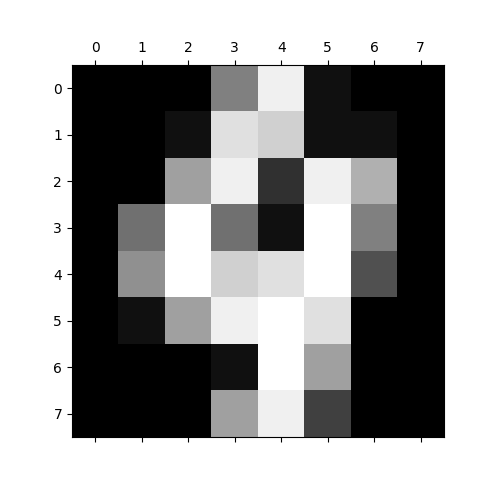
\includegraphics{mnist1.png}



All of the experiments that follow, unless stated otherwise, use a neural network with one hidden layer and the hyperbolic tangent function as activation function. We omit separate biases weights to simplify the presentation. It does not reduce the representational capacity of the model by too much because one of the hidden units can act as the bias by learning to represent a constant. The simplified model has two groups of weights,namely the input-to-hidden weights of dimension $N_{\text{in}} \times N_{\text{hidden}}$, and the hidden-to-output weights of dimension $N_{\text{hidden}} \times N_{\text{out}} $, where $N_{\text{in}},N_{\text{hidden}},N_{\text{out}}$, are the number of input covariates, hidden units and output units respectively. For example, for the simplified MNIST digits dataset described above, we have $N_{\text{in}} = 64 $ and $N_{\text{out}} = 10 $. 

Write down the explit likelihood.


For high dimensional models like BNNs, especially ones where no one-dimensional quantities should be predomimant apriori, like a network with standard normal prior, for example, the usual strategy of monitoring trace plots for diagnosing convergence is infeasible because it would require the user to skim through the traceplots for the thousands of parameters for even a moderately sized network. Therefore, instead we use multiple chains to compute Gelman's effective sample size (ESS) and monitor the minimum and median ESS over all parameters. The minimum ESS would indicate to us if any marginal quantities have slow convergence whereas the median would be indicative of the general speed of convergence of the chains as a whole. High ESS is desired as they imply low autocorrelation between samples, which means the Markov chain is moving rapidly across the parameter space and is generating more independent samples.

\section{Comparison with Early Stopping Committees}

In the first experiment we compare a Bayesian neural network to an early stopping committee of neural networks, a frequentist framework which is commonly used as a baseline method. Early stopping is an optimization technique in which training is stopped when the predictive accuracy on a holdout validate set ceases to improve. A group of neural networks initialized with different random seeds, after training by early stopping,  would then combine their predictions by simple averaging. We can find the results of the simulation in table \ref{esc}. We see that for smaller sized committees the predictive performance is significantly worse than Bayesian networks. However, with increasing size their predictive accuracy eventually matches that of BNNs. The target neural network is a single-hidden-layer network with 35 hidden units, where a standard normal prior has been placed on all weights. 

To sample from the BNN, a XHMC sampler with a diagonal metric and $\delta = 0.1$ is used. The step size and covariance metric are adapted for the first 1000 iterations with the target acceptance rate set to $0.9$. Four parallel chains each of length 2000 are sampled, resulting in 4000 final samples.
\begin{table}[]
\centering
\begin{tabular}{@{}rlllll@{}}
\multicolumn{1}{l}{}                            & \multicolumn{5}{c}{Test Error$\%$} \\ \midrule
Method\textbackslash{}Number of ensemble points & 2    & 5   & 10  & 100 & 1000 \\ \midrule
Early Stopping Committee of NNs                 & 91.2  & 88.6 & 47.0 & 51.6 & 19.2  \\ \midrule
BNN                                             & \multicolumn{5}{c}{23.4}        \\ \bottomrule
\end{tabular}
\caption{Compare the predictive accuracy of a Bayesian neural network with early stopping committees of neural networks of different sizes.}
\label{esc}
\end{table}

\section{GNUTS v.s. XHMC}
In the following experiment we compare the generalized NUTS termination criterion and the exhaustive termination criterion (XHMC). For both samplers we adapt the step sizes and the diagonal metric and use multiple chains like the previous experiment. We tested different values of the threshold $\delta$ and found that XHMC is capable of generating samples about as efficiently as GNUTS. 

\begin{table}[]
\centering
\begin{tabular}{@{}llll@{}}
\toprule
          & Test Error$\%$ & Min ESS & Median ESS \\ \midrule
XHMC $\delta=0.01$  & 25.6       & 681     & 1330       \\ \midrule
XHMC$\delta=0.05$  & 25.8       & 738     & 1346       \\ \midrule
XHMC $\delta=0.1$ & 28.6       & 396     & 1351       \\ \midrule
XHMC $\delta=0.2$ & 23.4       & 822    & 1324        \\ \midrule
GNUTS     & 26.0       & 682     & 1369       \\ \bottomrule
\end{tabular}
\caption{XHMC vs GNUTS}
\label{my-label}
\end{table}


\section{Gibbs Sampling v.s. Joint Sampling for Hyperparameter }

Next, we compare Gibbs sampling with joint sampling for a neural network with a Normal-Inverse-Gamma prior put on the input-hidden weights. A standard normal prior is put on the hidden-out weights. More specifically, we assume 
\[W_{ij} \sim \mathcal{N}(0,\sigma^2), \sigma^{-2} \sim \text{Gamma}(0.5,0.5), \]

which is equivalent to a student-t prior of degree 1 on $W_{ij}$. Both centered (CP) and non-centered (NCP) parameterizations are tried for joint sampling. For the Gibbs sampler, a GNUTS sampler with an identity covariance metric and a conservative step size $\epsilon = 0.01$ is chosen to sample the lower level weights. For joint sampling with both parametrizations, the step sizes and covariance metrics are tuned similarly as in previous experiments.

Focusing only on the variance parameter $\sigma^2$, we see that the CP encounters difficulty during sampling and results in a too low ESS for meaningful inference. In comparison the NCP encounters much less difficulty and has a reasonable ESS relative to the total number of samples. Compared to the  estimates generated by Gibbs sampling, joint sampling gives much higher ESS both for the hyperparameter and the lower-level weights. We tried different step sizes the lower-level weights in the Gibbs sampler but failed to find one that gives decent predictive accuracy and sample efficiency. This simulation shows that joint sampling and automatic step size tuning is an even bigger necessity than previously expected for sampling from BNNs with hierarchical priors.

\begin{table}[]
\centering
\begin{tabular}{@{}lllll@{}}
\toprule
              & Test Error$\%$ & $\sigma^2$ ESS & Min ESS & Median ESS \\ \midrule
Gibbs sampler & 88.4        & 4.38         & 1.29      & 45.3       \\ \midrule
Joint sampler- CP     & 25.8      & 4.86       & 4.69     & 1037         \\ \midrule
Joint sampler - NCP   & 28.4      & 504         & 434     & 1333        \\ \bottomrule
\end{tabular}
\caption{Compare Gibbs Sampling with Joint sampling for the hyperparameter. Note how the centered parametrization has low ESS for $\sigma^2 $ but high ESS in general, translating to good predictive accuracy. }
\label{my-label}
\end{table}

\section{Priors}

The horseshoe prior can be applied two ways on the weights in a layer. The first is to consider the weights as one long vector and assign the prior as one would in a regression problem. The second is an ARD-type approach, where a local variance is assigned for each hidden unit and one global variance for the entire layer. More specifically, suppose the layer in question has $n$ input units and $m$ hidden units. Then, the horseshoe ARD prior can be defined as follows 
\begin{align*}
& W_{i,\cdot} \sim \mathcal{N}(0,\lambda_i^2\tau^2) , \forall i \sim \{1,\dots, m \} \\
& \lambda_i \sim C^+(0,1) \\
& \tau \sim C^+(0,1), \\
\end{align*}
where $ W_{i,\cdot}  $ are the weights entering the $i$'th hidden unit. This is how the horseshoe prior was used for model selection in \cite{ghosh2017model}. Similarly we can define the regularized horseshoe ARD prior as 
\begin{align*}
& W_{i,\cdot} \sim \mathcal{N}(0,\tilde{\lambda}_i^2\tau^2) , \, \tilde{\lambda}_j^2 = \frac{c^2 \lambda_j^2}{c^2 + \tau^2 \lambda_j^2}  \forall i \sim \{1,\dots, m \} \\
& \lambda_i \sim C^+(0,1) \\
& \tau \sim C^+(0,1) \\
&c^2 \sim \text{Inv-Gamma}(2,8).\\
\end{align*}
We found that while the regularized horseshoe prior performs better than the original horseshoe prior in terms of having zero divergent transitions, none of the horseshoe priors can be said to induce great sampling efficiency, as both result in models whose posterior distribution are difficult to sample, resulting in low ESS. What's more is that even the Normal-Inverse-Gamma prior does not give better predictive performance than the standard normal prior, which we have already seen in earlier experiments comparing Gibbs sampling to joint sampling for the hyperparameter. 
\begin{table}[]
\centering
\begin{tabular}{@{}rrrrrrrr@{}}
\toprule
              & Normal & Normal-Inv-Gamma & Normal ARD     & RHS     & RHS ARD & HS  & HS ARD \\ \midrule
Test Error$\%$    & 23.4    & 26.8    & 24.0& 37.8    & 30.8      & 41.0       & 33.6               \\ \midrule
Min ESS       & 358      & 440   & 574  & 151  & 334     & 4       & 349              \\ \midrule
Median ESS    & 1348      & 1298  & 1220  & 911 & 1356     & 80      & 1354             \\ \midrule
\end{tabular}
\caption{Compare different priors: more complicated hierarchical priors do not necessarily give better predictive accuracy.}
\label{my-label}
\end{table}

\section{SGHMC}
The SGHMC has several extra tuning parameters other than the step size $\epsilon$ and number of leapfrogs $L$ that it inherits from the original HMC sampler. To reduce the number of parameters to tune, we fix these parameters ($\alpha=0.01, \hat{\beta}=0$) at the default values used in the experiments even though they are not sufficiently motivated. The parameters remain to be tuned are $\epsilon,L $ and $\eta$. We found that the SGHMC can perform similarly to the HMC although it requires having the right tuning parameter. Because the Metropolis acceptance step is omitted, there is no mechanism to avoid the chain from diverging into a low probability zone in the parameter space. Note that $L=50$ seems to give the best predictive accuracy regardless of the step size, this is puzzling because the $\epsilon$'s span 4 orders of magnitude and thus gives a wide range of integration time $t = \epsilon L$. The role of the learning rate $\eta$ is unclear other than that too large a $\eta$ seems to cause divergence (denoted by NA in the tables) more often. We see that SGHMC can generate samples that have good predictive performance, but their is no clear way to tune all the different hyperparameters other than by a grid search.


\begin{table}[]
\begin{minipage}{0.5\linewidth}
\centering
\footnotesize
\begin{tabular}{@{}lllll@{}}
\toprule
\multicolumn{5}{c}{Test Error$\%$}                  \\ \midrule
     & $\eta = 0.1$ & $\eta = 0.01$ & $\eta = 0.001$ & $\eta =0.0001$ \\ \midrule
     
$L=10$  & NA       & NA     & 72.2      & 84.4    \\ \midrule
$L=50 $ & 14.8       & 96.6     & 97.6      & 93.4    \\ \midrule
$L=100$  & 34.2      & 20.4    & 47.7     &  89.2  \\ \midrule
$L =200 $ & 46.8      & 37.2   & 92.4      & 87   \\ \bottomrule
\end{tabular}
\caption{SGHMC $\epsilon = 0.1$}
\end{minipage}
\begin{minipage}{0.5\linewidth}
\centering
\footnotesize
\begin{tabular}{@{}lllll@{}}
\toprule
\multicolumn{5}{c}{Test error$\%$}                  \\ \midrule
     & $\eta = 0.1$ & $\eta = 0.01$ & $\eta = 0.001$ & $\eta =0.0001$ \\ \midrule
$L=10$  & NA       & NA     & 68.8     & 84.2    \\ \midrule
$L=50$  & 14.8      & 93.8    & 97.2     & 91.4  \\ \midrule
$L =100$ & 37.2      & 20   & 44.4      & 89.2   \\ \midrule
$L=200 $ & 45.6      & 35.6     & 94      & 85.6   \\ \bottomrule
\end{tabular}
\caption{SGHMC $\epsilon = 0.01$}
\end{minipage}
\begin{minipage}{0.5\linewidth}
\centering
\footnotesize
\begin{tabular}{@{}lllll@{}}
\toprule
\multicolumn{5}{c}{Test Error$\%$}                  \\ \midrule
     & $\eta = 0.1$ & $\eta = 0.01 $& $\eta = 0.001$ & $\eta =0.0001$ \\ \midrule
$L=10$  & NA       & NA     & 68.8      & 89.8    \\ \midrule
$L=50$  & 15.4      & 95.4    & 97.8     & 95  \\ \midrule
$L =100$ & 34.2      & 25.0   & 46.8      & 91   \\ \midrule
$L=200 $ & 54.6      & 46.2     & 97.0      & 88.0   \\ \bottomrule
\end{tabular}
\caption{SGHMC $\epsilon = 0.001$}
\end{minipage}
\begin{minipage}{0.5\linewidth}
\centering
\footnotesize
\begin{tabular}{@{}lllll@{}}
\toprule
\multicolumn{5}{c}{Test Error$\%$}                  \\ \midrule
     & $\eta = 0.1 $ & $\eta = 0.01$ & $\eta = 0.001$ & $\eta =0.0001$ \\ \midrule
$L=10$  & NA       & NA     & 71.6      & 88.0    \\ \midrule
$L=50$  & 15.4      & 93.4    & 96.8     & 88.2  \\ \midrule
$L =100 $& 32      & 21.8   & 45.0      & 88.8   \\ \midrule
$L=200 $ & 53      & 39.4     & 95.4      & 78.4   \\ \bottomrule
\end{tabular}
\caption{SGHMC $\epsilon = 0.0001$}
\end{minipage}
\end{table}


\section{Scaled Priors}
In this experiment, we compared two normal priors with fixed variances. One is fixed at 1, the other at $\frac{1}{N_{\text{hidden}}}$. While we found little difference in their ESS's, the predictive accuracy from the standard normal prior is clearly better. It suggests

\begin{table}[]
\centering
\begin{tabular}{@{}llll@{}}
\toprule
            & Test Error$\%$ & Min ESS & Median ESS \\ \midrule
Hidden units = 35 & 23.4 (64.2)        & 358 (683)     & 1348 (1337)       \\ \midrule
Hidden units = 50 & 22.8 (65.0)        & 952 (66)      & 1358 (1348)         \\ \midrule
Hidden units = 65 & 22.0 (69.6)      & 610 (660)      & 1352 (1324)        \\ \bottomrule
\end{tabular}
\caption{Scaled v.s. Unscaled Priors. The figures in brackets are the results for the scaled priors. }

\end{table}

\section{Covariance Adaptation}
Here we explore whether its necessary or indeed useful to condition the HMC by the full covariance matrix of the target distribution. We experimented with a number of different priors and found that not only is adapting the full matrix more time consuming because of the need to multiply by a full mass matrix at every leapfrog step, the samples generated have much higher autocorrelation (equivalent to low ESS) to the point it slows sampling to a halt and destroys any hope of meaningful inference. We attribute this result to the singular nature of neural network models. For each of the prior, we sample from the posterior using the full covariance (dense metric), only the diagonal variances (diagonal metric) and no conditioning (unity metric) respectively. We see that the unity and diagonal metric performs similarly with the diagonal metric giving higher ESS's for the hierarchical priors, and they both take about the same time to compute.

\begin{table}[]
\footnotesize
\begin{tabular}{@{}lllll@{}}
\toprule
                     & Test Error$\%$ & Min ESS & median ESS & Compute Time \\ \midrule
Normal               & 67.0 (24.4) [20.6]   & 5 (563) [708] & 17 (1331) [1324]  & 36596 (10165) [11569]     \\ \midrule
Normal-Inv-Gamma     & 86.2 (22.4) [26.0]  & 4 (453) [378]  & 1271 (1348) [1271]    & 38095 (9234) [9158]     \\ \midrule
Normal-Inv-Gamma ARD & 91.2 (23.2) [27.2]  & 4 (370) [140]  & 8 (1295) [1332]    & 74326 (34940) [33212]     \\ \bottomrule
\end{tabular}
\caption{Covariance Adaptation. The figures in round brackets are generated by diagonal metrics, those in square brackets by unity metrics, and those not in brackets by dense metrics. }
\label{my-label}
\end{table}

\section{Number of Layers}
Now we fix the prior to be a standard normal distribution and vary the number of hidden layers. We found no evidence of increasing sampling difficulty with increased number of layers. 
However, for the the model with 4 hidden layers the test error went up significantly even though the ESS's stay about the same. 

\begin{table}[]
\centering
\begin{tabular}{@{}lllll@{}}
\toprule
            & Test Error$\%$ & Min ESS & Median ESS & Dimension \\ \midrule
Num Layers = 2 & 16.4    & 284 & 1596       & 12        \\ \midrule
Num Layers = 3  & 16.8  & 246 & 1418     & 12        \\ \midrule
Num Layers = 4  & 49.8  & 402 & 1310    & 12        \\ \bottomrule
\end{tabular}
\caption{Results on the effects of the number of hidden layers}
\label{my-label}
\end{table}

\section{Float v.s. Double Precision}
The following two experiments compare single and double precision for HMC sampling on a neural network model. The first experiment looks at the stability of the leapfrog trajectory. First, a number of points from the posterior distribution are generated by a sampler in double precision, which are then each augmented by an independent momentum drawn from a standard normal distribution. Then the list of $(q_i,p_i)$ points are cast into single precision. The two sets of points are then integrated forward for a fixed number of iterations with a reasonably conservative step size and we compare the difference in Hamiltonian between the start and end point of the trajectory. We found that for the normal prior the final states in trajectory differ in energy by less than $10^{-5}$ and for the normal-inv-gamma prior the difference on the order $10^{-2}$, which translates to at most a difference of 1 $\%$ in the final acceptance rate.

The second experiment looks at the differences in test error. 


In both experiments we did not find a significant difference between the two, suggesting that the transition to single precision should not harm predictive accuracy and correctness. 

\begin{table}[]
\centering
\begin{tabular}{@{}rll@{}}
\toprule
\multicolumn{1}{l}{} & Float & \multicolumn{1}{r}{Double} \\ \midrule
Normal               & 27.6   & 25.8                         \\ \midrule
Normal-Inv-Gamma     & 23.2  & 28.8                         \\ \bottomrule
\end{tabular}
\caption{Difference in test error ($\%$) between single and double precision.}
\end{table}

\section{Static  v.s. Dynmaic HMC}
In the following experiment we ran two HMC samplers, the regular HMC and windowed HMC, over a grid of tuning parameter values $(\epsilon,L)$, and compare the samples generated by the best combination with those generated by the dynamic HMC (NUTS). The model is a single-hidden-layer BNN with a standard normal prior.
The step sizes and covariance metrics are tuned automatically as in previous experiments. The results show that the static samplers has similar performance as the dynamic sampler, both in terms of predictive accuracy and ESS. Although this may be more indicative of the success of the dual averaging tuning of the step size $\epsilon$ in generating stable leapfrog trajectories. 


The sampling performance and predictive accuracy seems to be independent of the number of leapfrog steps, and also of the use or not of the windowed sampler. 
\begin{table}[]
\centering
\begin{tabular}{@{}llll@{}}
\toprule
        & Test Error$\%$ & Min ESS & Median ESS \\ \midrule
$L = 10 $  & 22.8 (22.2)    & 704 (283) & 1061(765)       \\ \midrule
$L = 50 $  & 27.0 (24.2)  & 36 (196)  & 379 (1533)     \\ \midrule
$L = 100  $  & 28.6 (23.8)  & 126 (254)  & 823 (1256)    \\ \midrule
$L = 200  $   & 22.2 (24.0)    & 713 (340)      & 1196 (1204)         \\ \midrule
$L = 500   $ & 23.8  (23.4)       & 345 (693)      & 1245  (1252)        \\ \midrule
Dynamic & 23.4         & 358       & 1348         \\ \bottomrule 
\end{tabular}
\caption{Static vs Dynamics HMC. The figures in brackets are generated by windowed HMC}
\label{my-label}
\end{table}

\section{WAIC for Model Selection}
Next, we would test the WAIC's ability to select the number of hidden units in a single hidden-layer neural network model. The true test error is estimated by a holdout test set. Different numbers of hidden units are tested and their WAIC computed by dynamic HMC. According to theory, the model with the lowest WAIC should be chosen to minimize predictive error.
We found that the model with the lowest WAIC does not match those selected by holdout test error. The failure of the WAIC to select the best model might be explained by the poor mixing of the importance sampler when estimating the WAIC, which was noted in a review of predictive checks for Bayesian inference \cite{vehtari2017practical} . 


\begin{table}[]
\centering
\begin{tabular}{@{}lllll@{}}
\toprule
               & WAIC & Test Error$\%$ & Min ESS & Median ESS      \\ \midrule
Number of Hidden Units = 35    & $3.05 \times 10^4$  & 23.4    & 358 & 1348   \\ \midrule
Number of Hidden Units = 50  & $4.35 \times 10^4$   & 20.4  & 714  & 1342                \\ \midrule
Number of Hidden Units = 75 &$ 6.36 \times 10^4$   & 21.2  & 883  & 1351                 \\ \midrule
Number of Hidden Units = 90 &$ 7.57 \times 10^4$  & 21.2   & 562  & 1359                 \\ \bottomrule
\end{tabular}
\caption{WAIC for model selection}
\label{my-label}
\end{table}


\section{Conclusion}

Experimenting on a simplified MNIST dataset, we found that Bayesian neural networks can achieve about the same and sometimes better predictive accuracy than early stopping committees. The main difference between the two is that early stopping committees need to be manually  tuned to achieve decent accuracy, whereas BNNs can achieve the same with dynamic HMC and automatic tuning of step sizes and covariance metrics. 

Based on experiments conducting on this dataset, we can make the following observations.

\begin{enumerate}
\item XHMC can perform as well as GNUTS, $\delta = 0.1$ seems like a good default value. We recommend XHMC since it requires fewer computations. 

\item Gibbs Sampler can be difficult to tune and we prefer joint sampling and the non-centered parametrization for sampling for hierarchical priors.

\item Standard normal prior works better than complicated hierarchical priors or "informed priors" that take model structure into account when setting the scale.

\item Automatic tuning of step size and covariance metric is essential for a robust sampling workflow. Diagonal metric should be chosen over dense metric.

\item WAIC does not work so well at choosing the best model as the theory suggests. 

\item Single precision is good enough for HMC sampling with BNNs. 

\item  SGHMC can can give similar performance as HMC but the result is not robust to choice of tuning parameters.

\item Integration time does no seem to influence predictive accuracy or sample quality, once the step size is chose so that acceptance rate is kept high.

\end{enumerate}

Finally, results above make should make one skeptical about claims made about Bayesian neural networks, since they defy some traditional wisdom about statistics. For example, for overparametrized models where the dimension is much larer than the number of observations, one should use hierarchical priors like the horseshoe to perform regularization. However, our experiments show that such regularization often harms predictive accuracy, even when there is high ESS overall.



\chapter{Conclusion}
use xhmc, unscaled normal prior, 
use diag e 
don't use sghmc
don't use waic 
can use float on gpu

\chapter{Model}

\section{Markov Chain Monte Carlo}




\cite{green2015bayesian} gives a good summary of dynamical MCMC methods (langevin diffusion,MALA,HMC) and related convergence assessment methodologies.

In the late 80s and throughout the 90s, Bayesian statistical modeling became
feasible for a much larger class of problems than previously thought possible,
because of the availability of abundant computing power. Much work was produced
in MCMC methodologies\cite{robert2013monte}, theory\cite{tierney1994markov,roberts2004general} as well as in applications thereof.  



See more about Bayesian data analysis in \cite{gelman2014bayesian}. 


Evaluate sample quality
Effective sample size is defined as 
\[ ESS = N \{ 1 + 2 \sum_k \gamma(k) \}^{-1}, \]

estimated by the initial
monotone sequence estimator \cite{geyer1992practical}

It is a useful metric for measuring quality of the samples obtained from a
Markov Chain. We can take the mean or minimum ESS across all covariates.

Convergence diagnostics for high-dimensional target distributions. Theoretically, need convergence of the Markov Chain to the joint distribution, in practice only convergence to marginal distributions are checked. The literature has only looked at applying univariate diagnostics to each parameter individually and then calculate some summary statistic (mean,min) or carry out multiple testing if the diagnostic is based on a hypothesis test.

KL-divergence can be used to compare samples drawn from two different samplers.
The method advanced in \cite{boltz2007knn,boltz2007high} uses a kernel estimator to estimate the KL divergence between two empiricial distributions. The curse of dimensionality makes it difficult for application to high-dimensional posterior distributions $p(\theta|x)$, however, we can apply it to marginal predictive distributions $p(y|D)$ which usually are low-dimensional, when the covariates $x$ are fixed.

Tune MCMC algorithms. MCMC algorithms usually have a small number of tuning
parameters, such as a stepsize $\epsilon$, the number of leapfrog steps, or more
basic quantities like the length of the chain. Classic Bayesian methodology
\cite{robert2013monte} uses a mix of visual inspection of trace plots and
numerical convergence diagnostics like ESS as discussed earlier. The process
requires human intervention each time an algorithm is run and tuning parameters
readjusted after the diagnostics are computed. 


\section{ Hamiltonian Monte Carlo }. 

Originally developed in the physics community \cite{duane1987hybrid},
Hamilotnian Monte Carlo was introduced to the statistics community by Neal
\cite{neal2012bayesian}, 
by way of Computer Science, through his work on inference for Bayesian neural
networks. It was shown to be very efficient in sampling from high-dimensional
distributions and was used in the framework of bayesian inference to achieve superior predictive
performance in machine learning tasks\cite{guyon2004result}. However, its sensitivity to tuning parameters, relative difficulty of
implementation, and a lack of accessible
exposition to its theory, itself a subject of open research, precludes
widespread adoption. While some of these challenges remain to this day, the development of STAN \cite{carpenter2016stan} has made it significantly easier to carry out Bayesian inference with HMC, and is the main reason for increasing adoption of HMC in applications (cite statistics). Meanwhile, the invention Riemmanian Manifold Hamiltonian Monte Carlo (RMHMC) \cite{girolami2011riemann}, which exploits differential geometry to aid in local adaptation of the HMC sampler, and subsequent exploration the ideas introducd in the their paper, lead to better understanding of the mathematics behind HMC \cite{livingstone2016geometric,betancourt2014geometric} and  improvements to the sampler \cite{betancourt2013generalizing,betancourt2013general}. Many of these new developments have been and will be included in the STAN language. STAN also eliminates the need for tuning HMC. Users of STAN are shielded from the implementation details and tuning parameters settings, required only to specifiy the distributions involved in the models. 

Since STAN is so central to the present HMC literature, we would explain how it functions in the following exposition. Before that, however, we would explain the basic version of HMC on which STAN is built and to which many extensions are added. 












Now, STAN has many tiny yet crucial tricks which form part of the adaptive
tuning and diagnostic mechanism. Bear in mind that Bayesian inference with STAN is not completely
automatic because judgement still has to be made upon reviewing the results of
the returned samples to determine if they are valid. And like traditional MCMC
diagnostics this judgement is not completely objective in the sense that there
are no metrics that come with theoretical guarantees. 





Another problem with the above approach is that it is only unsuitable when the
target distribution can be approximately linearly transformed into a
distribution which can be easily explored by a standard HMC sampler.If the target
distribution has more complicated geometry that might differ in
curvature in various parts of its support, a constant $M$ is not enough to ensure
effective decorrelation during sampling. This motivates the use of
a location-dependent mass matrix $M(x)$ and is called the Riemannian Hamiltonian
Monte Carlo. More on this later. 






Note to preserve the correct invariant distribution, the calculation of the
potential energy function in the Hastings ratio must be done exactly. In later
discussion of stochastic gradient HMC sampler and extensions, we see data
subsamlping being combined with stochastic optimization to yield 
randomly varying the trajectory length is a recommended part of standard HMC
methodology. 

HMC is invariant to rotation.
Randomly choose stepsize. 
Shortcut method.
Mapping Multivariate Gaussian distribution. width of the distribution in the most constrained direction. Square root of the smallest eigenvalue of the covariance matrix for q.
Quote: HMC is valid as long as the dynamics is simulated using a method thatis reversible and volume-preserving. 

Tuning the HMC is tricky: for optimal stepsize see \cite{beskos2013optimal}

Understanding of optimal HMC stepsize, number of leapfrogs steps, number of leapfrog steps to reach nearly independent points.
Ex: Grows as $O(d^{1/4})$.







Symplectic  = volume-preserving


\section{Neural networks} 



\section{MCMC methods applied to hierarchical models}
\begin{enumerate}
\item Centered vs uncentered parametrization in hierarchical models.







\section{approximate inference for fast training and prediction}


Finally, there is the simple idea of approximating the the posterior
distribution by fitting a gaussian density around the posterior mode, this is
known as Laplace's method. It is first applied to BNNs by Mackay in \cite{mackay1992evidence}. In \cite{vivarelli2001comparing}, the author compared the predictive performance of Laplces's method against HMC and found the latter to perform slightly better, with more marked improvement on smaller datasets. An interesting point to note about this method is that by using a Gaussian approximation we have to calculate its covariance matrix by using the Hessian. Since neural network models are actually singular the Hessian is not positive definite everywhere and adjustments have to be made to make it work. In \cite{hernandez2015probabilistic} the authors compared Laplace's method with several approximate inference methods as well as HMC and found it to perform less well than the others. However, they constrained the covariance matrix of the Gaussian approximation to be diagonal to save computational time. Understandibly this leads to worse approximation. On the other hand, one is not forced to choose between a diagonal covariance or the full-rank one. Quasi-newton approximations are possible, and fits neatly within the optimization pipeline.

Variationa inference for bayesian neural networks started with the work of \cite{hinton1993keeping}, who developed a variational inference algorithm using the language of information theory. He used the concept of minimizing the description length of the weight, which is equivalent to minimizing the KL divergence as described above. 

Graves' work \cite{graves2011practical} built on the the Hinton's paper and introduced a stochastic gradient variational method. However, the stochastic gradient estimates are biased and the prior is limited to be Gaussian. In \cite{blundell2015weight} this is further improved upon using the re-parametrization trick \cite{opper2009variational,kingma2013auto,rezende2014stochastic}. This yields the Bayes by Backprops (BBB) algorithm.

The Expectation propogation (EP) approach to approximate inference in BNNs was experimented in \cite{jylanki2014expectation} but saw little follow-up because they method the authors developed was batch-only and could not scale to large datasets.A stochastic version was designed by \cite{hernandez2015probabilistic}, called the Probabilistic Backpropogation (PBP), and was shown to perform well on a wide range of test datasets. However, it has the limitation of being applicable only to regression problems. In \cite{ghosh2016assumed} it is extended to multiclass classification problems through a monte carlo approximation. 

In Myshkov et al's submission to a NIPS workshop (cite), the authors analyzed the performance of a few approximate inference algorithms for BNNs against the "gold-standard" that is the HMC, among those tested were PBP and EP. And they did not perform too poorly against MCMC methods. More analysis of this work to come later.  

In Bayesian dark knowlege, we also try to minimize the KL divergence, but do so
in a way that compresses model knowledge.  

Why do we assume the prior distribution of weight parameters to be normal centered at 0?

Study of prior distributions in neural networks.\cite{lampinen2001bayesian,titterington2004bayesian}

\section{Scaling MCMC methods to large datasets}




Expectation propogation. Original paper\cite{minka2001expectation}, Gelman and collegues wrote a paper on it \cite{gelman2014expectation}

Stochastic version discussed here \cite{li2015stochastic}
See also \cite{dehaene2015expectation} for another study of expectation propogation in the large sample size context. 

A stochastic natural gradient extension has been devised and applied to bayesian neural network models \cite{teh2015distributed}
Probabilistic Backpropogation is a special case of SEP applied to Bayesian neural networks \cite{hernandez2015probabilistic}.


Laplace Approximation. It is based on the second order approximation of the
log-likelihood of the posterior density around its mode.

Suppose the log posterior density $f(x)$ has a mode at $x^*$, then near $x^*$ we
have 
\[ f(x) = f(x^*) + \nabla f(x)|_{x=x^*} (x-x^*) + \frac{1}{2} (x-x^*)^TH(x-x^*)
\]
where $H$ is the Hessian matrix of $f(x)$ evaluated at $f(x)$, that is,
\[ H_{ij} = \frac{\partial^2 f(x)}{\partial x_i \partial x_j }|_{x=x^*} \]




\section{Bayesian Model Selection and Prediction}


\section{Multiple Modes}

Neural network models are known to have multiple modes, although it is widely believed that most local modes have similar likelihood values to the global mode. In Neal's work on bayesian neural network, he also assumed that multimodality would not cause any problems in inference and in prediction. 


Insert pseudocode. 
\chapter{Experimeints}
Plan:
Collect problems on which to fit neural networks of modest size. 

Example 1: Mackay's robot arm's data. 

This is a regression problem where the data is generated as follows:
\[ y_1 = 2.0 * \cos(x_1) + 1.3 \cos(x_1+x_2) + z_1 \]
\[ y_2 = 2.0 * \sin(x_1) + 1.3 \sin(x_1+x_2) + z_2 \]
where $z_1,z_2$ are independent Gaussian random variables of standard deviation
$0.05$ and $x_1$ is uniformly generated from $[-1.932,-0.453]\cup
[0.453,1.932]$, and $x_2$ is uniformly generated from the range $[0.534,3.142]$.
200 training cases and 200 test cases were generated according to the equations
above. 

A neural network with a single hidden-layer of 16 hidden units was used to model
the data.

Bayesian logistic regression with hierarchical prior. Following \cite{zhang2014semi}

1. Sample weights with HMC, sample hyperparameter with Gibbs sampling.

2. Same as above with Windowed update.

3. Same as 1 but with tempering. 

4. Sample weights and hyperparameter together with HMC. (STAN)

5. Softabs 

6. Empirical fisher information matrix 
Compare ESS/L.
Data: Same classification problem datasets from the RHMC paper \cite{girolami2011riemann}, as well as simulated data.
Funnel problem
Compare ESS/L as well as marginal distribution of the hyperparameter, which is known in this case. 

Bayesian neural network of more than 2 hidden units and of 1 hidden layer only. Test 1 layer network of 100 units with fixed normal prior and hierarchical prior.
Data: Same regression problem datasets from the PBP paper \cite{hernandez2015probabilistic}. 


For all the above problems it is straight forward to adapt code to compare manual hyperaparameter tuning with automatic tuning by STAN and by bayesian optimization. Compare ESS/L results for the final parameters selected. 

Test robustness of consensus mcmc to poor mixing. Split data into a $K$ subsets randomly, $K$ being a manageable small number (5 or 8), then tune some posterior distribution samplers to mix well and some others don't. Test on both regular and singular models.
 
For neural networks being used to fit a small number of observations relative to its dimension, there is a problem of overfitting. In \cite{gal2015bayesian}, it was shown that approximate bayesian inference via dropout helps to mitigate this problem. We argue that MCMC sampling would achieve even better performance.

Use only a small percentage (5 or 10 percent) of the MNIST dataset and perform batch inference with BNN. Try both fixed prior and hierarchical priors. Use the best sampler found from earlier experiments. 
Compare with gradient descent and dropout. 

Done with MCMC
Bayesian model selection. 
Bayesian neural networks can also be used to model data when the size of the training set is small. In this setting frequentist training of neural networks suffers from overfitting. Practioners who use neural network would like to make predictions for new data $\{x_{new}\}$. In principle, before making predictions the practioner should first decide on the model(s) to be used to fit the training data. While bayesian model averaging (BMA) is an interesting idea which promises to improve prediction accuracy, assignign prior to different models is difficult to justify and may appear arbritary. More importantly, for large models the time and memory complexity required to sample from the posterior distribution or the variational approximation thereof, as well as sample from the predictive distribution, would quickly become unmanageable as the number of models increases. 

For this reason, model selection is usually carried out, where a model is selected and then trained to make predictions on new data. Because there are infinitely many combinations of different tuning parameters and model structure paramters, an exhaustive search is impossible and instead a heuristic combinations of tuning paramters are chosen to form the candidtate models. Usually a holdout set (test set) is used to estimate the predictive performance of the model on new data. The model with the lowest average predictive error is then chosen. 

In bayesian statistics \cite{gelman2014bayesian} cross-validation, especially leave-one-out cross-validatino is recommended for model selection. It comes with a high computational cost, but remains the most principally sound method for estimating the out-of-sample log predictive density. WAIC(Widely applicable information criterion) is derived using singularity learning theory and estimates consistently the loocv, even for singular models. Traditional information criteria like AIC, BIC and DIC relies on the the asymptotic normality of the mle, which only holds if the Fisher information matrix is non-singular at the mle. While the justification of WAIC relies on heavy algebraic machinery, to apply it only requires being able to draw samples from the posterior distribution under a model and evaluate the likelihood.  
In the machine learning/deep learning community, model selection is usually done
by comparing the predictive accuracies of the different trained models on a
holdout set. The usual justification of this practice is that if the dataset
exhibits enough data redundancy then  this is enough to estimate the test
accuracy. However, this is certainly dependent on the particular dataset and the
size of the model one would like to use to fit the data. The most statistically
principled practice would be too use all available data to train models and then
select the best model using cross-validation. Efficeint approximation to the
cross-validation log density like the WAIC is therefore deemed desirable for
model selection. 

An important statistical question is therefore as follows: for neural network models, is
the use of a holdout set for model selection consistent with best practice?
That is, do these two methods make the same model selection decision ? What happens
in the small data regime? I suspect the utitilty of WAIC would be the greatest
in small-to-medium data size settings, where a randomly chosen subset that is 25
percent the size of total dataset is unlikely to estimate the test error with a
low variance (unbiased by highly variable).

Approximation inference. 
Compare PBP, BBB, LA, to HMC and SGD. Use fixed prior. Test effect of small training
set. Compare time to reach test accuracy. Use importance sampling to calculate
WAIC. Decrease memory until these approximation methods perform better than
MCMC.

Scaling MCMC
SGLD, SGHMC, pSGLD, SGFS, Thermostat. Compare test accuracy with batch HMC.
Tuning by test accuracy, or tuning by ESJD.

Consensus MCMC 
See if singularity severely degrades quality of classification.

Effects of pruning
In the BBB paper, performance does not degrade drastically even if 98 percent of
the weights are removed. See same thing applies to MCMC samples. 





But before all this can start we first need to overcome the difficulties of
sampling from the posterior distribution of a bayesian neural network. The
first source of difficulty comes from the correlation in the posterior distribution induced by
the connection between neurons in consecutive layers. Each neuron in a layer is
connected to all neurons from the previous layer and hence is influenced by
values in the previous layer. This is the first source of correlation. The
second source of correlation comes from the use of a hierarchical prior on the
weights of the network. This is tackled by Riemmanina Manifold type MCMC
methods, which make use of information of the second derivatives of the
log-posterior. The trade-off is now a linear system of full rank must be solved
to calculate each update in the markov chain. This has the time complexity of
$O(p^3)$ which makes it difficult to apply to neural network models, who's
expressiveness comes from its large number of parameters. 

Posterior correlation due to hierarchical prior vs inter-layer correlation. 

The second source of difficulty comes from the cost of evaluating the
log-posterior density and its derivative with respect to the parameters. For
exact calculation, both requires going through the entire dataset. In
frequentist fitting of neural networks, this problem is bypassed by evaluating
the gradient using a random subset of the original datapoints as input. The mcmc
analogues are stochastic gradient mcmc methods. These methods, however, suffer
from slow mixing in the case of SGLD variants, and the need to do matrix
inversion in the case of SGHMC variants. Interesting compromise can be made by
replacing the full fisher information matrix by a diagonal matrix or low-rank
approximations. 

And other obstacle prevents the widespread adoption of mcmc for inference in BNN
is the dependance on GPUs for calculating the gradient of the weights by
backpropogation. GPUs make fast calculation of gradient of networks with
increasing number of layers feasible, however its downside is its limited
fast-access memory. Transferring weights from the GPU to the main disk creates a
bottleneck in the calculation that balances out the speed gain. Even if we
disregard the problem with speed and only focuses on the memory, we find that
bayesian inference by mcmc as carried out traditionally by the statistics
community, where a large number of samples from the chain is generated and
saved, diagnosced for convergence and then quantities where expectation is taken
with respect to the posterior distribution are approximated by taking
expectation with respect to the empirical distribution instead. The first
problem with this approach is the lack of tool for assessing convergence for
high-dimensional distributions. Convergence of every marginal distribution does
not imply convergence of the joint distribution. Also, it is impossible to
visually inspect
the trace plot of all covariates along the chain in order to assess convergence,
depriving ourselves one of the more reliable tools in the classical mcmc
methodology. Another problem with the traditional methodology is the necessity
to compute a long chain (even after thinning) and use the samples for expectaion
calculation. No matter how decorrelated the samples from the chain are,
more than a handful of samples at a time is required to calculate an unbiased
estimate of the expectation that doesn't suffer from high variance. This limits
the size of the network that can be trained, often it precludes the use of a GPU
altogether and limit us to shallow networks. A frequentist training of neural
network only $O(p)$ memory is required to store the weights in memory, but in
the bayesian framework described above $O(pT)$ memory is required, where $T$ is
the number of samples from the chain that we wish to retain. In many
applications a large
model of 1 million paramters is found to minimize the test error on a holdout
set among many possible model structure. One might then wish to assign prior to
weights in this network and carry out bayesian inference. Even assuming there is
enough memory on the GPU, it is reasonable to assume that in most applications it might not be worth the 50 times increase in memory
budget to improve predictive accuracy by 2 percent. 

Since neural networks are 
mostly used for predictive purposes and there is little interpretability in the
posterior distribution of the individual weights, which are
always integrated out to find the predictive distribution anyway, one might find
it worthwhile to look at approximate inference methods that aim to find
an approximation to the posterior distribution with a tractable distribution and
which allows for easy calculation of the posterior predictive distribution. 

One note that to calculate the WAIC, the memory requirement is only $O(nT)$,
where $n$ is the number of observations and $T$ the number of mcmc samples. This
inspires the methdology of bayesian model selection and inference. First we
choose the model by using the most efficient mcmc methods. Since evaluation of
the WAIC is independent of the dimension of the model, this can be done on the
GPU and enjoy the speed up that it provides. Once the model is chosen,
approximation inference is carried out to fit an approximate model that allows
fast training and prediction, with most variations using $O(p)$ memory.

While batch version of HMC is not practical because of size constraints, for
research purposes or small data problem it might be necessary to simulate a
markov chain that is as targeting as close the posterior distribution as
possible, excluding stochastic gradient versions where bias is introduced by
dropping the metropolis correction step. A comparative study of the effectivenss the new
RMHMC type samplers applied to jointly sample the weights and hyperparameters is
long due. 

Make the connection between natural gradient learning and riemannian manifold
hmc



What is the largest neural networks that can be trained by modern hardware using 1996 techniques (HMC tuned by heuristics plus windowed state) from Neal's thesis?  

How good are the samples generated using these techniques? Look at min effective sample size across all covariates. Trace plot of randomly selected components/ hyperparameters. Should see skewed distribution. Plot it.


Train models of moderate size first (can fit on harddisk, most likely 1 hidden layer), then apply Riemman Hamiltonian Monte Carlo to see if you get much better results. Also compare that to just normal approximation around max. Multiple mode seems to be a problem. But also have result(heuristics) from frequentist results saying that local min is not a serious problem cuz most local modes are similar cost value. 

Sample using MALA, then Riemann MALA.

The langevin dynamics algorithm has fewer tuning parameters, but mixes slower. Hope is that Riemann MALA is a compromise between MALA and full HMC. 

Compare different metrics used in RHMC. 

How much does initialization matters. i.e. Initialize to random normal covariates vs variance-matching initialization. See Xavier initialization: 
\[X \sim U[- \sqrt{\frac{6}{n_{in}+n_{out}}}, \sqrt{\frac{6}{n_{in}+n_{out}}}] \]

Compare predictive accuracy reached under fixed time budget.

Simulation studies: 

Target distribution: multivariate student-t distribution. Zero mean and diagonal covariance with common variance. See Jake Baker's master's thesis.His simulations don't stress the samplers as much as I'd wish. For example the highest dimension tested was 20. 

He used the KL divergence as performance metric, calculated as follows \cite{boltz2007high}. 

Since we care about prediction, we can follow Mykshov by comparing different MCMC samplers/approximate bayesian inference using the KL divergence of the predictive distribution with the $x$ integrated out instead. First, this is usually a one dimensional distribution, which makes much more sense when we are using kernel methods to approximate the KL divergence anyway.

Funnel distribution: typical of bayesian models with hierarchical priors. Neal has used slice sampling and HMC to draw from it. Betancourt used Riemmanian HMC with his metric. 

Hasn't been done: MALA, RMALA, HMC with partial momentum, windowed,
semi-separable HMC (benchmark),RHMC with softabs(hasn't been a comparison of
ESS) adaptive HMC (Gaussian process) each of the HMC variety above can also be

coupled with the trick in \cite{burda2011bayesian} (fix conditioning matrix
between each sample).
Experiment with efficient diagonal approximation to covariance matrix.

Hierarchical bayesian logistic regression: Methods above as well as stochastic
gradient MCMC (sgld,pre-conditioned sgld, thermostat,sghmc)
Try on simulated data as well as benchmark datasets.


Bayesian dark knowledge: how does the quality of the MCMC samples from the
posterior distribution of the teacher model affect the approximation of the
prediction distribution by the student neural network. How sensitive is it?


Memory efficient implementation of MCMC.
Keep history of random seeds for mv normals, as well as history of acceptance
decision.
Given only $\theta_T$, can reproduce chain $\{\theta_1, \dots, \theta_T \}$ on
command.
Useful for GPU implementations of MCMC.
Predictive performance(cross-validation) used for adaptive
tuning\cite{wang2013adaptive}


Using predictive performance as metric to tune MCMC. i.e. select tuning
parameters that give the highest average posterior predictive density for new
data or highest accuracy on test set.

Compare variational posterior to true posterior.  

Statistical question: compare the train/test holdout metric to WAIC. Do they
give the same conclusions?\cite{kohavi1995study}
Try k-fold cross-validation as well.

Evaluate variational models in terms of WAIC. 

Work using evidence aka marginal likelihood for neural network model comparison. 
\section{ neural networks}
Previous work:\cite{blundell2015weight}

Suppose the dimension $p$ of $\theta$ is so high that we can only afford to keep 20 copies or so of $\theta$ in memory (on a GPU, for example). 
What is the best practice (MCMC vs variational inference) for bayesian inference in this scenario. 

Effect of number of layers on autocorrelation.(with or without hierarchical prior).

Model selection as follows: select certain quantities to monitor convergence (hyperparameters, acceptance ratio etc), store values needed to calculate WAIC, select model. Then use approximate inference (variational inference or expectation propogation) to compute approximation to predictive distribution for predictions.

Sgmcmc: how many minibatches of data should be used to update the main paramters before switching to sampling hyperparameters? In sghmc, they have examples where the entire dataset is passed through and the other just some data.
Goal: 

stochastic gradient quasi netwon langevin dynamics requires extra tuning paramters with little guidance on how to tune them \cite{csimcsekli2016stochastic}

preconditioned sgld introduces bias\cite{li2015preconditioned}.
\bibliographystyle{plain}

\end{enumerate}
\bibliography{test}
\end{document}
